% This must be in the first 5 lines to tell arXiv to use pdfLaTeX, which is strongly recommended.
\pdfoutput=1
% In particular, the hyperref package requires pdfLaTeX in order to break URLs across lines.
\newif\ifreview \newcommand{\review}{\reviewtrue}
\newif\ifarxiv \newcommand{\arxiv}{\arxivtrue}
\newif\ifcamera \newcommand{\cameraready}{\cameratrue}

\arxiv

\documentclass[11pt]{article}

% Change "review" to "final" to generate the final (sometimes called camera-ready) version.
% Change to "preprint" to generate a non-anonymous version with page numbers.
% \usepackage[review]{acl}

\ifreview \usepackage[review]{acl} \fi
\ifarxiv \usepackage[final]{acl} \fi
\ifcamera \usepackage[final]{acl} \fi

% Standard package includes
\usepackage{times}
\usepackage{latexsym}
% For proper rendering and hyphenation of words containing Latin characters (including in bib files)
\usepackage[T1]{fontenc}
% For Vietnamese characters
% \usepackage[T5]{fontenc}
% See https://www.latex-project.org/help/documentation/encguide.pdf for other character sets

% This assumes your files are encoded as UTF8
\usepackage[utf8]{inputenc}

% This is not strictly necessary, and may be commented out,
% but it will improve the layout of the manuscript,
% and will typically save some space.
\usepackage{microtype}

% This is also not strictly necessary and may be commented out.
% However, it will improve the aesthetics of text in
% the typewriter font.
\usepackage{inconsolata}

%%%%%%%%% CUSTOM PACKAGES %%%%%%%%%%

\usepackage{graphicx}
\usepackage{amsmath}
\usepackage{amssymb}
\usepackage{booktabs}
\usepackage{amsfonts}
\usepackage{algorithm}
\usepackage{algorithmicx}
\usepackage{algpseudocode}
\usepackage{footnote}

\usepackage{fancybox}
\usepackage{tcolorbox}

\usepackage{xcolor}
\usepackage{comment}
\usepackage{amsthm}
\usepackage{bbm} % indicator function
\usepackage{subcaption}
\usepackage{multirow}
\usepackage{comment}
\usepackage{makecell} %multiline cell
\usepackage{tabularx}
\usepackage[normalem]{ulem}
% \useunder{\uline}{\ul}{}
\usepackage{booktabs}
\usepackage[switch]{lineno}

\usepackage{url}
\usepackage{xspace}

\let\enumerate\compactenum 
\let\endenumerate\endcompactenum 
\let\description\compactdesc 

%%%%%%%%%%%%%%%%%%%%%%%%%%%%%%%%%%%%
% General
\newcommand{\nbf}[1]{{\noindent \textbf{#1}}}

\newcommand{\eat}[1]{}
\newcommand{\vsa}{\vspace*{-0.28cm}}
\newcommand{\vsb}{\vspace*{-0.19cm}}
\newcommand{\vsc}{\vspace*{-0.16cm}}
\newcommand{\cbit}{\begin{compactitem}}
\newcommand{\ceit}{\end{compactitem}}
\newcommand{\cben}{\begin{compactenum}}
\newcommand{\ceen}{\end{compactenum}}

\newenvironment{packed_enum}{
\begin{enumerate}
  \setlength{\itemsep}{1pt}
  \setlength{\parskip}{2pt}
  \setlength{\parsep}{0pt}
}{\end{enumerate}}

\DeclareMathOperator*{\argmax}{argmax}

\usepackage[capitalize]{cleveref}
\crefname{section}{Sec.}{Secs.}
\crefname{table}{Table}{Tables}
\crefname{figure}{Fig.}{Figs.}
\crefname{algocf}{alg.}{algs.}
\Crefname{algocf}{Algorithm}{Algorithms}

\definecolor{headercolor}{RGB}{240, 255, 240}
\definecolor{rowcolor1}{RGB}{255, 240, 240} %
\definecolor{rowcolor2}{RGB}{240, 240, 255}
\definecolor{rowcolor3}{rgb}{1,1,1}

\definecolor{pink1}{HTML}{FAD5D1}
\definecolor{pink2}{HTML}{EE9A8F}
\definecolor{pink3}{HTML}{C6464C}

\definecolor{blue1}{HTML}{A9B8ED}
\definecolor{blue2}{HTML}{7886CB}
\definecolor{blue3}{HTML}{4050B5}

\frenchspacing
\usepackage{soul}

\definecolor{customred}{rgb}{0.95, 0.35, 0.45}
\definecolor{customgreen}{rgb}{0.35, 0.75, 0.5}
\definecolor{customblue}{rgb}{0.35, 0.45, 0.95}

\newcommand{\benchname}{ToolBH\xspace}
\newcommand{\hlred}[1]{{\sethlcolor{customred}\hl{#1}}}
\newcommand{\hlgreen}[1]{{\sethlcolor{customgreen}\hl{#1}}}
\newcommand{\hlblue}[1]{{\sethlcolor{customblue}\hl{#1}}}



\def\paperTitle{
ToolBeHonest: A Multi-level Hallucination Diagnostic Benchmark for Tool-Augmented Large Language Models
}

\title{\paperTitle}

\def\authorBlock{
    Yuxiang Zhang$^\textnormal{1}$\footnotemark[1] \qquad
    Jing Chen$^\textnormal{2}$\footnotemark[1] \qquad
    Junjie Wang$^\textnormal{1}$\footnotemark[1] \qquad
    Yaxin Liu$^\textnormal{3}$ \\
    \textbf{
    Cheng Yang$^\textnormal{4}$ \qquad
    Chufan Shi$^\textnormal{3}$ \qquad
    Xinyu Zhu$^\textnormal{3}$ \qquad
    Zihao Lin$^\textnormal{5}$ \qquad
    Hanwen Wan$^\textnormal{6}$} \\
    \textbf{Yujiu Yang$^\textnormal{3}$ \qquad
    Tetsuya Sakai$^\textnormal{1}$ \qquad
    Tian Feng$^\textnormal{2}$\footnotemark[2] \qquad
    Hayato Yamana$^\textnormal{1}$\footnotemark[2]
    } \\
    $^\textnormal{1}$Waseda University \quad
    $^\textnormal{2}$Zhejiang University \quad
    $^\textnormal{3}$Tsinghua University \quad \\
    $^\textnormal{4}$CUHK \quad
    $^\textnormal{5}$Virginia Tech \quad
    $^\textnormal{6}$CUHK, Shenzhen \quad \\
    {\tt\small joel0495@asagi.waseda.jp} \quad 
    {\tt\small chenjing\_1984@zju.edu.cn} \quad 
    {\tt\small wjj1020181822@toki.waseda.jp} \quad \\
    {\tt\small t.feng@zju.edu.cn} \quad 
    {\tt\small yamana@yama.info.waseda.ac.jp} \\
    \tt\small\url{https://github.com/ToolBeHonest/ToolBeHonest}
}

\author{\authorBlock}

\begin{document}
\maketitle

{
  \renewcommand{\thefootnote}%
  {\fnsymbol{footnote}}
  \footnotetext[1]{Equal contribution.}
  \footnotetext[2]{Corresponding Author.}
}

\begin{abstract}
Tool-augmented large language models (LLMs) are rapidly being integrated into real-world applications. 
Due to the lack of benchmarks, the community has yet to fully understand the hallucination issues within these models.
To address this challenge, we introduce a comprehensive diagnostic benchmark, \benchname. 
Specifically, we assess the LLM's hallucinations through two perspectives: depth and breadth. 
In terms of depth, we propose a multi-level diagnostic process, including (1) solvability detection, (2) solution planning, and (3) missing-tool analysis. 
For breadth, we consider three scenarios based on the characteristics of the toolset: missing necessary tools, potential tools, and limited functionality tools. 
Furthermore, we developed seven tasks and collected $700$ evaluation samples through multiple rounds of manual annotation.
The results show the significant challenges presented by the \benchname benchmark. The current advanced models Gemini-1.5-Pro and GPT-4o only achieve total scores of $45.3$ and $37.0$, respectively, on a scale of $100$. 
In this benchmark, larger model parameters do not guarantee better performance; the training data and response strategies also play crucial roles in tool-enhanced LLM scenarios.
Our diagnostic analysis indicates that the primary reason for model errors lies in assessing task solvability.
Additionally, open-weight models suffer from performance drops with verbose replies, whereas proprietary models excel with longer reasoning. 
\end{abstract}

\section{Introduction}

To replicate human intelligence in artificial general intelligence (AGI), recent studies suggest that a promising solution is enabling large language models (LLMs) to use tools to handle diverse complex scenarios~\cite{DBLP:journals/corr/abs-2302-07842@aug-survey}. 
For instance, tool-augmented LLMs can employ various APIs or coding tools to tackle intricate tasks, such as mathematical reasoning.
However, as shown in~\cref{fig:intro-examples}, several hallucinatory phenomena arise when these LLMs attempt to use tools. 
Specifically, the LLMs might utilize the wrong tools or offer solutions with non-existent tools.
This occurs because LLMs cannot discern whether a problem is solvable with the tools at hand, and instead, they use fictitious tools, hindering progress in developing AGI models.
Therefore, a pressing issue is \textit{assessing the hallucination phenomenon when LLMs utilize tools}.

\begin{figure}[!tp]
\centering
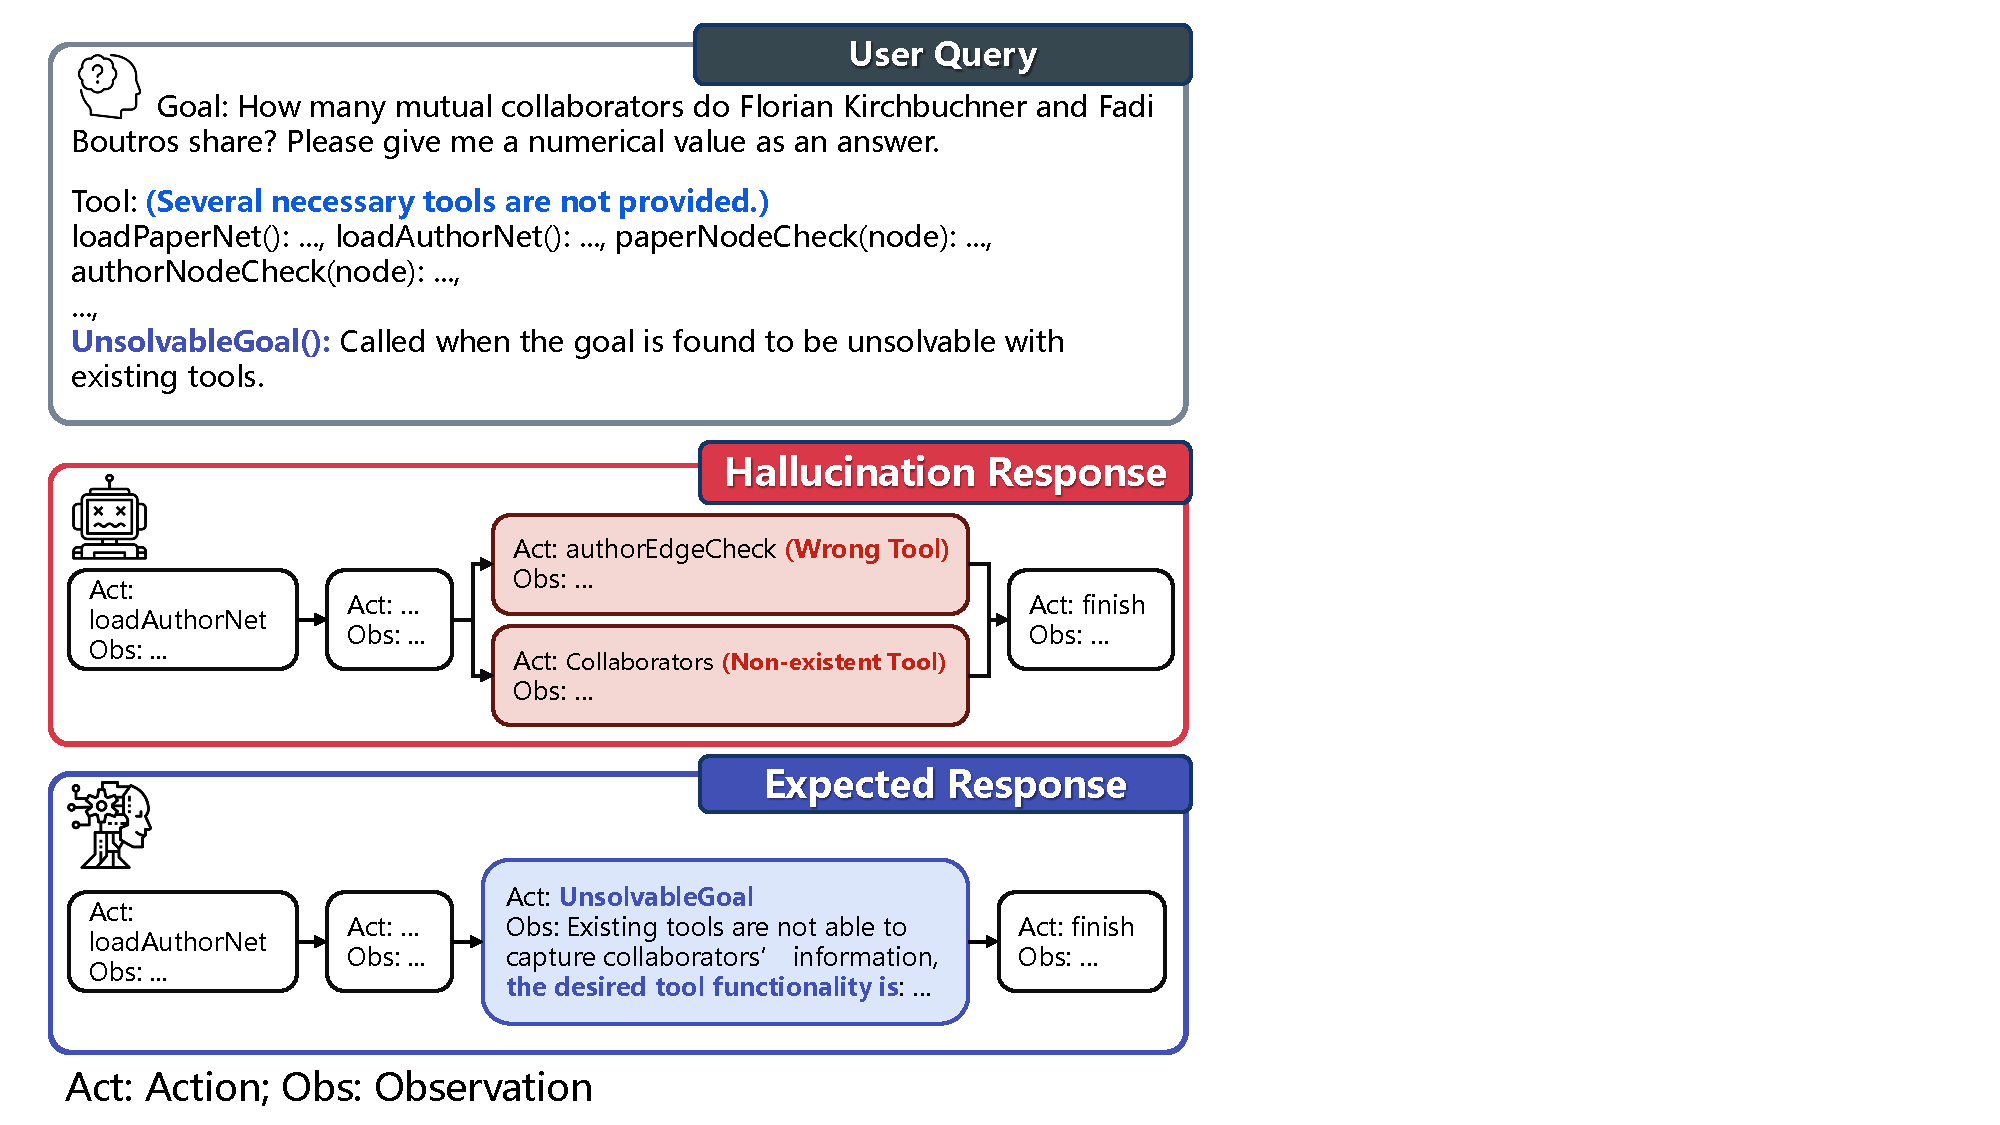
\includegraphics[width=0.48\textwidth]{figures/examples0614_new.pdf}
\caption{
Hallucinations (\hlred{red}) and expectations (\hlblue{blue}) of the LLM's response to the use of the task for tools that do not have a correct answer.
The problem example is taken from the AgentBoard~\cite{DBLP:journals/corr/abs-2401-13178@agentboard} Tool-Query dataset, tested with ChatGPT~\cite{openaichatgpt@chatgpt}.
Wrong Tool reflects a common situation where LLM uses a provided wrong tool as the final answer;
Non-existent Tool, on the other hand, is an example of hallucination.}
\vspace{-1em}
\label{fig:intro-examples}
\end{figure}

However, current benchmarks for tool-based tasks presuppose the provision of complete and usable tools by users, primarily focusing on evaluating how LLMs utilize these tools~\cite{DBLP:journals/corr/abs-2308-03688@agentbench,DBLP:journals/corr/abs-2307-16789@toolbench,DBLP:journals/corr/abs-2401-13178@agentboard}. 
For example, AgentBench~\cite{DBLP:journals/corr/abs-2308-03688@agentbench} and ToolBench~\cite{DBLP:journals/corr/abs-2307-16789@toolbench} aim to introduce a broad array of tasks, and AgentBoard~\cite{DBLP:journals/corr/abs-2401-13178@agentboard} evaluate the multi-step tool planning abilities of these models.
Although MetaTool~\cite{DBLP:journals/corr/abs-2310-03128@metatool} considers incomplete lists of tools provided by users, it still focuses solely on determining whether a task can be completed.
Therefore, to ensure a comprehensive evaluation of the various hallucinatory phenomena in tool usage, we develop the \benchname benchmark.
It is a multi-level hallucination diagnostic benchmark for tool-augmented LLMs. 
Inspired by medical diagnostic procedures~\cite{Wu2023Establishment@medical} and existing hallucination benchmarks~\cite{DBLP:journals/csur/JiLFYSXIBMF23@survey-hallu-1,DBLP:conf/acl/LiuZBMSCD22@survey-hallu-2}, \benchname systematically assesses hallucinations from perspectives of \textbf{depth and breadth} (Details in~\cref{benchmark}).

In the assessment of hallucination \textbf{depth}, we introduce a multi-level diagnostic procedure framework that incorporates \textit{(1) solvability detection}, \textit{(2) solution planning}, and \textit{(3) missing-tool analysis}.
The solvability detection task assesses whether the user query can be addressed with the given toolset. 
Subsequently, the solution planning task requires the LLM to propose a plan of tools tailored to address the task sequentially. 
In the end, the missing-tool analysis task builds upon its predecessor by requiring the LLM to delineate how the tools address the specific demands in each step. 
For tasks considered unsolvable, the LLM is tasked with identifying and elaborating on the functionalities of the missing tools, thereby offering insights to aid in completing the toolkit.
On the side of \textbf{breadth}, we consider three critical scenarios from the perspective of toolset features: missing necessary tools, potential tools, and limited functionality tools.
Furthermore, we design seven tasks across these scenarios, including iterative calls and optimal tool selection tasks.
Finally, we collect $700$ samples (user query, tool set, solution) across $7$ tasks through multiple rounds of human annotations and establish an evaluation metric for each diagnostic task (Details in~\cref{ss:multi-level-evaluation}).

We conduct experiments on $14$ LLMs using the \benchname benchmark, which includes $7$ proprietary and $7$ open-weight models.
Our analysis reveals that despite some open-weight models achieving competitive performance compared to proprietary counterparts in general tasks~\cite{2023@open-llm-leaderboard,2023@opencompass}, they exhibit substantial gaps in unsolvable scenarios presented by the \benchname benchmark. 
Notably, the best-performing open-weight model, Llama-3-70B, still trails behind the proprietary models, with only $32\%$ of the total score of Gemini-1.5-Pro~\cite{DBLP:journals/corr/abs-2403-05530@gemini-1.5} and $40\%$ of GPT-4o~\cite{openai@gpt4o}, indicating considerable room for improvement in open-weight models.
A detailed error analysis shows a variety of error patterns.
Proprietary models tend to exhibit fewer instances of using non-existent tools, suggesting better tool recognition capabilities.
However, they also showed higher rates of instrumental reasoning errors, reflecting problems comprehending the task's solution sequence and reasoning logic.
On the other hand, open-weight models suffer more from solvability hallucinations, often misjudging the complexity and feasibility of tasks. This highlights a critical area for enhancement in model reasoning.

Our findings demonstrate the significance of the \benchname benchmark in identifying and addressing deficiencies in LLMs. 
The benchmark provides detailed analysis and valuable insights into specific error patterns under unsolvable LLM tool usage scenarios, offering guidance for future research.

\section{Related Work}
\label{related-work}
\subsection{Tool-based Benchmarks}

Recent advancements in LLMs have highlighted their potential when augmented with external tools, prompting the development of several benchmarks to assess their tool-using capabilities.
For example, benchmarks such as API-Bank~\cite{DBLP:conf/emnlp/LiZ000YLHL23@apibank}, ToolBench~\cite{DBLP:journals/corr/abs-2307-16789@toolbench}, AgentBench~\cite{DBLP:journals/corr/abs-2308-03688@agentbench} and AgentBoard~\cite{DBLP:journals/corr/abs-2401-13178@agentboard} evaluate LLMs' capabilities in planning, retrieving, and calling APIs across various tasks.
Moreover, ToolQA~\cite{DBLP:conf/nips/ZhuangYWSZ23@toolqa} introduces a dataset for assessing tool-using LLMs through question answering, distinguishing between internal knowledge and external tool usage.
However, these benchmarks operate under a stringent assumption: users will provide a list comprising all requisite tools and describe each explicitly. 
This assumption rarely holds true in real-world scenarios. 
Few benchmarks~\cite{DBLP:journals/corr/abs-2310-03128@metatool} incorporate a reliability test, which evaluates whether the model can appropriately return ``None'' when necessary tools are absent from the list. 
This approach fails to address significant gaps, such as exploring the reasons behind the output of ``None''.
To address these challenges, we introduce \benchname, a comprehensive multi-level hallucination diagnostic benchmark. 
\benchname evaluates the tool-using capabilities of models across diverse scenarios and further investigating hallucinations to assist the community in identifying underlying causes.

\subsection{Evaluating Hallucinations in LLMs}

In LLMs, hallucination occurs when the output is inconsistent with the input, contradicts established knowledge, or cannot be verified against factual data~\cite{DBLP:journals/corr/abs-2309-01219@hallu-survey,li2024surveyhonestylargelanguage@hallu_survey}. 
This phenomenon challenges the reliability and credibility of LLMs, especially in real-world applications.

To evaluate such hallucinations, current benchmarks are introduced that focus on the discriminative and generative capacities of LLMs.
For instance, TruthfulQA~\cite{DBLP:conf/acl/LinHE22@truthfulqa} evaluates the truthfulness of generated responses. 
In assessing the ability to differentiate between real and hallucinatory statements, HaluEval~\cite{DBLP:conf/emnlp/LiCZNW23@halueval} focuses on whether the model can accurately identify hallucinatory content within state information.
Moreover, FACTOR~\cite{DBLP:conf/eacl/MuhlgayRMLRBALSS24@factor} investigates whether the model tends to assign higher likelihoods to factual statements over non-factual ones, examining the bias toward recognizing truth.
However, these benchmarks solely assess the knowledge of large models without considering the interaction with tools.
Therefore, referencing their generative and discriminative approaches, as well as the methods used in coding~\cite{DBLP:conf/emnlp/ZhuYCLLY23@hallu_cite1} and medical diagnosis~\cite{Wu2023Establishment@medical}, we propose a multi-level benchmark to explore the phenomena of hallucinations in the tool-augmented LLMs.

\section{The \benchname Benchmark}
\label{benchmark}

\begin{figure*}[!tp]
\centering
\includegraphics[width=1.0\textwidth]{figures/mainfigure_6.14_new.pdf}
\caption{The pipeline of \benchname benchmark. In-breadth, we examine three scenarios (MNT, PT, LFT) that could induce hallucinations from the perspective of the toolset. We employ an in-depth, multi-level evaluation (solvability detection, solution planning, and missing-tool analysis) to diagnose the reasons for hallucinations in LLM.}
\label{fig:main_process}
\vspace{-1em}
\end{figure*}

\subsection{Design Philosophy}

To comprehensively assess the hallucination phenomena encountered by tool-enhanced large models, we design tasks and data processing procedures from both the depth and breadth perspectives of hallucination evaluation. 
Accordingly, our workflow adheres to the following design philosophy:
\begin{itemize}
\setlength{\itemsep}{1pt}
\setlength{\parskip}{2pt}
\setlength{\parsep}{0pt}
\item Unsolvability in real-world tasks.
\item In-depth: Multi-level hallucination diagnosis.
\item In-breadth: Hallucination-inducing scenarios.
\end{itemize}

\nbf{Unsolvability in real-world tasks.} 
In our observations of real-world applications, hallucinations frequently occur when LLMs attempt to address tool-use requests that they believe are solvable but are inherently unsolvable. 
We summarize these instances as \textit{unsolvable long-tail tool-using tasks}.

\nbf{Multi-level hallucination diagnosis.}
Our aim is to conduct an in-depth analysis of hallucinations experienced by LLMs when tackling unsolvable tasks to explore the underlying mechanisms. 
To achieve this objective, we decompose these unsolvable tasks into three progressive stages. 
This decomposition is based on the level of detail in the responses, as detailed in~\cref{ss:multi-level-evaluation}.


\nbf{Hallucination-inducing scenarios.}
In tool-based tasks, the pivotal element is the tool-related information, including toolsets and tool descriptions. 
Therefore, we consider two hallucination-inducing scenarios from the perspective of tool characteristics (Details in~\cref{benchmark:hallu_scena}).

Following these guidelines, we introduce an unsolvable long-tail robustness assessment benchmark to diagnose hallucinations comprehensively and at multiple levels.

\subsection{In-depth: Multi-level Diagnostic Task}
\label{ss:multi-level-evaluation}

Based on unsolvable tool-using problems, we design a three-level diagnostic task framework: (1) solvability detection, (2) solution planning, and (3) missing-tool analysis.
As shown in~\cref{fig:main_process}, we employ distinct metrics for each level.  We present the rationale for implementing a multi-level evaluation framework in~\cref{append:necessity-multi-level}.

\subsubsection{Level-1: Solvability Detection}
At the first level, the LLM assesses whether a task is solvable from a macro-level perspective. 
Specifically, by referencing the provided toolset, the model must comprehend the user query and the tool descriptions, then determine and indicate whether the task is solvable or unsolvable.
We tackle this task as a binary classification task and utilize the exact match (EM) as the metric.

\subsubsection{Level-2: Solution Planning}

Given that many queries require collaboration between multiple tools for completion, we explore the model's planning capabilities from a micro-level perspective. 
Specifically, the model divides user requests into sub-goals, utilizing the corresponding tools in each step.
Additionally, we introduce an ``UnsolvableQuery'' tool to address situations where the available tools cannot achieve the sub-goals.
Inspired by the Precision\@k set retrieval evaluation measure, we design a new progress rate (PR) metric, which assesses the accuracy of a predicted tool sequence ($P$) based on the ground truth ranking ($G$).
Specifically, PR compares each predicted tool name ($p_i$) against the corresponding ground truth tool name ($g_i$), terminating the comparison at the first mismatch and treating all subsequent tools as incorrect. 
The metric for each sample is defined as follows:

\begin{equation}
\textstyle 
\text{PR} = \frac{\sum_{i=1}^{\min(k-1, |G|)} \mathbf{1}(p_i = g_i)}{|G|},
\end{equation}
where indicator function \(\mathbf{1}(p_i = g_i)\) returns $1$ for a match and $0$ otherwise.
$k$ is the index of the first mismatch between \( P \) and \( G \). If there is no mismatch (i.e., \( P \) matches \( G \) completely), let \( k \) be equal to \( |G| + 1 \), which essentially points to one position beyond the last tool in \( G \).

\subsubsection{Level-3: Missing-Tool Analysis}
Building on the requirements of level-2, this task requires LLM candidates to provide a detailed account of the rationale behind each subtask. 
Specifically, for sub-goals deemed unsolvable, the model must articulate the functions of absent tools in detail, enabling further evaluation of its reasoning ability.
Therefore, we include two metrics: progress rate (PR) and matching score (MS).
While the PR metric remains consistent with Level-2, its application in Level-3 serves distinct purposes. It enables the investigation of hallucination risks in ReAct~\cite{DBLP:conf/iclr/YaoZYDSN023@react} agent reasoning for unsolvable tool tasks and evaluates model consistency across tasks with varying context lengths.

For MS, we consider a text-matching method for each sample. 
If the model identifies ``UnsolvableQuery'' in each sub-goal, it outputs a predicted description ($d_u$) of the tool's functionality.
Inspired by widely-used tool-matching algorithms~\cite{DBLP:journals/corr/abs-2310-03128@metatool,DBLP:conf/nips/ZhuangYWSZ23@toolqa}, we develop a tool database that contains tool names and their descriptions. 
Initially, the algorithm uses $d_u$ to search the most similar tool description from the database. 
If the retrieved description matches the golden description, the MS score for this sub-goal is awarded a perfect score of $1.0$.
If a match is not found, $d_u$ and the golden description are encoded into embeddings using an embedding model, namely $emb_u$ and $emb_g$. 
In this paper, we use the \texttt{all-MiniLM-L6-v2}~\cite{DBLP:conf/acl/WangBHDW21@minilmv2} as the embedding model.
Subsequently, the cosine similarity between these embeddings is computed.
The process can be summarized by the equation below:
\begin{equation}
\textstyle
\text{MS}_\mathrm{sub-goal} = 
\begin{cases} 
1.0 & \text{if matched} \\
\frac{emb_u^T \cdot emb_g}{\|emb_u\| \|emb_g\|} & \text{otherwise}
\end{cases}
\end{equation}

Finally, we compute the arithmetic mean of $\text{MS}_\mathrm{sub-goal}$ across each sample's sub-goal.

\subsection{In-breadth: Tool-based Hallucination-inducing Tasks}
\label{benchmark:hallu_scena}

In breadth, we divide tool-using scenarios into three categories based on tool characteristics: missing necessary tools (MNT), potential tools (PT), and limited functionality tools (LFT).
In this section, we present an overview of each scenario and its subtasks.

\subsubsection{Missing Necessary Tools (MNT)}
The task becomes unsolvable when a toolset lacks the necessary tools for task completion.
Under these conditions, LLMs might engage in hallucinatory behavior, such as invoking non-existent tools. 
To generate unsolvable tasks, we remove a randomly chosen tool from the ground truth list.
In this scenario, we consider subtasks based on the number of steps needed to complete the task:

\noindent{1. Single-step tool utilization:} Completing the task with one tool.

\noindent{2. Multi-step tool utilization:} Using multiple tools, categorized into: ``Without Repetition'' (No tool is reused) and ``With Repetition'' (Some tools are used multiple times).


\subsubsection{Potential Tools (PT)}

In addition to the provided tools, some user queries may involve specific environments like operating systems (OS) and websites (Web).
These environments may contain potential tools not specified in user requests, making their use impermissible. 
However, LLMs may inappropriately exploit these tools. 
In this scenario, we construct unsolvable tasks by removing a randomly golden tool and adding environment details to mislead the LLM to use non-provided or inappropriate tools.
We consider the following subtasks:

\noindent{1. OS:} Tasks may prompt the LLM to assume it is within an OS environment, where it might consider system commands like ``rm'' and ``ufw'' to solve the task. The misuse of such commands could lead to serious consequences.

\noindent{2. Web:} Similarly, the LLM might be induced to use web technologies (e.g., JavaScript, SQL).


\subsubsection{Limited Functionality Tools (LFT)}

LFT scenarios involve correct tools with functional limitations. 
Unsolvable tasks are generated by adding extra requirements or constraints to queries, task descriptions, or tools.
We include the following subtasks:

\noindent{1. Iterative:} These mimic multi-functional tools requiring different functions at each step. Unsolvable tasks are created by removing a required function. For example, using tools like HanLP~\cite{he-choi-2021-stem@hanlp}, different models are needed for various requirements. An unsolvable task requires a function not listed.

\noindent{2. Optimal tool selection:} These scenarios involve multiple similar-function tools where only one meets all requirements. Unsolvable tasks are created by making requirements more stringent. For instance, a task might need a specific minority language translation with strict computing resource requirements, which no tool can fully satisfy.

\subsection{Data Curation}
\label{ss:data-curation}

Aligned with our design principles, we introduce a multi-turn annotation process, including four key steps: (1) creating seed samples, (2) synthesizing samples, (3) filtering, and (4) constructing data samples.
The details are in~\cref{append:details-benchmark}, including prompts, filtering criteria and other details.
An overview follows:

\nbf{(1) Creating seed samples.} Considering the subtasks outlined in~\cref{benchmark:hallu_scena}, a series of seed samples are constructed, each comprising a triplet (user query, toolset, golden solution). These samples are created for different scenarios and subtasks that fit our definition of these terms and are validated by multiple team members.

\nbf{(2) Synthesizing samples.} 
We design prompt templates for each subtask (details in~\cref{append:generation_prompt}).
After that, we insert the seed samples into these templates and synthesize additional samples using advanced LLMs: Gemini-1.0-Pro~\cite{DBLP:journals/corr/abs-2312-11805@gemini-1.0} and GPT-4o~\cite{openai@gpt4o}. 

\nbf{(3) Filtering.} 
Initially, the synthesized data are filtered based on similarity to seed samples to ensure diversity, using an embedding model~\cite{DBLP:conf/acl/WangBHDW21@minilmv2} for semantic similarity and manual checks for task similarity.
Moreover, our team manually reviews and removes low-quality or biased samples, such as those containing errors or specific political biases. 
The detailed criteria are described in~\cref{append:filter-criteria}.

\begin{table*}[tp]
\setlength{\tabcolsep}{3pt}
\small
\centering
\caption{Statistics of \benchname benchmark.}
\label{tab:key_statistic}
\vspace{-1em}
\resizebox{\textwidth}{!}{
\begin{tabular}{l|rrr|rr|rr|r}
\toprule
\multicolumn{1}{l|}{Scenario} & \multicolumn{3}{c|}{Missing Necessary Tools}                                          & \multicolumn{2}{c|}{Potential tools} &  \multicolumn{2}{c|}{Limited Functionality Tools} & \multicolumn{1}{c}{Overall} \\
\midrule
Subtask                   & Single-step  & \makecell[c]{Multi-step \\ w/o Repetition} & \makecell[c]{Multi-step \\ w/ Repetition} & \hspace{-1em}OS                   & \hspace{-1em}Web                   & \makecell[c]{Iterative}                      & \hspace{3.5em}\makecell[c]{Optimal \\ Selection}  & - \\
\midrule
Length of User Query (Avg.)   & 364.1 & 449.5 & 476.2 & 412.9 & 450.2 & 471.6 & 525.0 & 449.9         \\
\# of Tools Provided (Avg.)        & 4.3 & 6.0 & 6.0 & 4.2 & 6.1 & 5.5 & 5.9 & 5.4          \\
\# of Tools Used (Avg.)        & 2.0 & 5.8 & 6.8 & 3.9 & 5.3 & 5.6 & 2.0 & 4.5          \\
\# of Unsolvable Tools (Avg.)        & 1.0 & 1.0 & 2.0 & 1.0 & 1.0 & 1.1 & 1.0 & 1.2            \\ \midrule
\# of Samples (Solvable)          & 50                     & 50                        & 50                       & 50                   & 50                    & 50                             & 50                     & 350              \\ 
\# of Samples (Unsolvable)       & 50                     & 50                        & 50                       & 50                   & 50                    & 50                             & 50                     & 350          \\
\bottomrule
\end{tabular}}
\end{table*}

\nbf{(4) Constructing data samples.} 
After filtering, our data pool is enriched with high-quality samples.
Subsequently, we randomly select fresh samples from this pool for the next round of annotation.

We conduct multiple annotation rounds until the number of samples meets our expectations.
Initially, four seed samples are manually created for each of seven subtasks. 
Through iterative refinement, each subtask ultimately contains $300$ unique samples.
Subsequently, we select the $100$ samples that exhibit the greatest variation, as determined by both the tool descriptions and the task contexts.
Further manual review then narrows these down to $50$ solvable and $50$ unsolvable samples for each of seven subtasks, resulting in a total of $700$ samples in our \benchname benchmark.

To enhance the comprehensiveness and utility of our benchmark, we have structured it into three levels of difficulty, ranging from Level-1 to Level-3. 
This hierarchical structure ensures that the benchmark can evaluate models across a spectrum of complexity. 
Each level contains an equal number of solvable and unsolvable samples, bringing the total number of test samples to $1,050$.
This aligns our benchmark with the scale of the most recent mainstream benchmarks~\cite{DBLP:journals/corr/abs-2307-16789@toolbench,DBLP:journals/corr/abs-2401-13178@agentboard,DBLP:journals/corr/abs-2308-03688@agentbench}.

\subsection{General Statistics}

\cref{tab:key_statistic} provides a comprehensive statistical analysis of the \benchname benchmark, featuring $700$ samples with solvable and unsolvable tasks across various scenarios.
It encompasses a range of indicators, including the number of tools provided, the number of tools utilized, and the average number of ``UnsolvableQuery'' tools used.
Moreover, we employ the Llama3~\cite{metaAI@llama3} tokenizer to measure the average length of the user queries.

\section{Experiments}
\label{experiment}
\subsection{Baselines}

We collect $14$ widely-used LLMs, comprising $7$ proprietary and $7$ open-weight models (Details in~\cref{append:experimental-setting}).

Specifically, seven proprietary models includes: Gemini-1.0-Pro~\cite{DBLP:journals/corr/abs-2312-11805@gemini-1.0}, Gemini-1.5-Pro~\cite{DBLP:journals/corr/abs-2403-05530@gemini-1.5}, GPT-3.5-Turbo~\cite{openaichatgpt@chatgpt}, GPT-4-Turbo~\cite{DBLP:journals/corr/abs-2303-08774@gpt4}, GPT-4-1106, GPT-4-0613 and GPT-4o~\cite{openai@gpt4o}.

Given the diversity of architectures in open-weight models, 
including dense and mixture-of-experts, we select seven widely used models:
Llama-3 series (Llama-3-8B-Instruct and Llama-3-70B-Instruct)~\cite{metaAI@llama3}, 
Llama-2 series (Llama-2-7B-Chat, Llama-2-13B-Chat, and Llama-2-70B-Chat)~\cite{DBLP:journals/corr/abs-2307-09288@llama2}, and Mistral series (Mistral-7B-Instruct~\cite{mistralai@7B} and Mixtral-8x7B-Instruct~\cite{mistralai@8x7B}).

\begin{table*}[tp]
\setlength{\tabcolsep}{3pt}
\small
\centering
\caption{The \benchname leaderboard with $14$ LLMs, with the best \textbf{bolded} and the second best scores \underline{underlined}.}
\label{tab:main_results}
\vspace{-1em}
\resizebox{\textwidth}{!}{
\begin{tabular}{l|cccc|cccc|cccc|c}
\toprule
\multirow{2.5}{*}{Model} & \multicolumn{4}{c|}{Missing Necessary Tools} & \multicolumn{4}{c|}{Potential Tools} & \multicolumn{4}{c|}{Limited Functionality Tools} & \multirow{2.5}{*}{Overall} \\
\cmidrule{2-13} 
 & L1-EM & L2-PR & L3-PR & L3-MS & L1-EM & L2-PR & L3-PR & L3-MS & L1-EM & L2-PR & L3-PR & L3-MS &  \\
\midrule
\multicolumn{14}{c}{\textit{Proprietary}} \\
\midrule
GPT-3.5-Turbo &
16.0 & 19.1 & 15.6 & 21.0 & 5.0 & 11.4 & 11.6 & 14.0 & 33.0 & 3.0 & 1.4 & 0.2 & 13.4 \\
Gemini-1.0-Pro &
12.0 & 12.5 & \underline{41.2} & \underline{35.3} & 3.0 & 9.3 & \textbf{48.0} & \textbf{38.9} & 25.0 & 4.7 & 3.2 & 1.8 & 20.6 \\
GPT-4-0613 &
\underline{59.3} & 63.1 & 29.2 & 27.1 & 44.0 & 46.0 & 23.5 & 18.6 & 31.0 & 13.0 & 0.0 & 0.0 & 31.7 \\
GPT-4-1106 &
44.7 & 54.9 & 34.5 & 31.7 & 32.0 & 43.0 & 34.1 & 26.6 & 42.0 & \underline{26.0} & 1.5 & 1.2 & 32.5 \\
GPT-4-Turbo &
58.7 & \underline{70.3} & 28.2 & 25.4 & 45.0 & \underline{63.7} & 30.5 & 22.3 & 42.0 & 25.3 & 0.3 & 0.0 & 35.9 \\
GPT-4o &
53.3 & 69.9 & 24.8 & 24.8 & \underline{47.0} & 62.0 & 27.9 & 33.2 & \underline{56.0} & 21.9 & \underline{6.8} & \textbf{4.4} & \underline{37.0} \\
Gemini-1.5-Pro &
\textbf{62.7} & \textbf{70.7} & \textbf{42.8} & \textbf{36.6} & \textbf{56.0} & \textbf{68.6} & \underline{43.6} & \underline{38.2} & \textbf{69.0} & \textbf{27.1} & \textbf{8.5} & \underline{3.9} & \textbf{45.3} \\
\midrule
\multicolumn{14}{c}{\textit{Open-weight}} \\
\midrule
Llama-2-13B &
16.7 & 0.7 & 0.0 & 0.0 & 2.0 & 0.9 & 1.0 & 0.0 & 20.0 & 2.3 & 0.0 & 0.0 & 3.7 \\
Mixtral-8x7B &
4.0 & 13.5 & 1.4 & 1.3 & 0.0 & 8.2 & 2.0 & 2.0 & 18.0 & 6.5 & 0.0 & 0.0 & 4.8 \\
Llama-2-7B &
5.3 & 2.2 & 2.0 & 0.7 & 4.0 & 16.5 & 0.3 & 0.0 & \textbf{46.0} & \underline{7.7} & 0.5 & 0.0 & 6.5 \\
Llama-2-70B &
17.3 & \underline{14.4} & 2.0 & 0.4 & 2.0 & \underline{19.8} & 2.7 & 0.7 & 33.0 & 0.5 & 0.2 & 0.0 & 7.9 \\
Llama-3-8B &
13.3 & 4.0 & \textbf{7.0} & \textbf{6.1} & 7.0 & 4.5 & \underline{5.1} & \underline{2.9} & 45.0 & 2.0 & \underline{1.3} & \textbf{0.7} & 8.1 \\
Mistral-7B &
\underline{27.3} & 9.1 & 4.5 & 1.9 & \textbf{20.0} & 4.7 & 3.4 & 1.2 & 31.0 & \textbf{15.0} & \textbf{1.6} & \underline{0.3} & \underline{10.1} \\
Llama-3-70B &
\textbf{31.3} & \textbf{35.5} & \underline{4.8} & \underline{4.9} & \underline{19.0} & \textbf{23.6} & \textbf{5.2} & \textbf{4.3} & \underline{34.0} & 4.0 & 0.0 & 0.0 & \textbf{14.6} \\
\bottomrule
\end{tabular}}
% \vspace{-0.5em}
\end{table*}


% \begin{table*}[]
% \setlength{\tabcolsep}{3pt}
% \small
% \centering
% \caption{main results.}
% \begin{tabular}{c|cccc|cccc|cccc|c}
% \toprule
% \multicolumn{1}{c|}{Scenario} & \multicolumn{4}{c|}{Missing Necessary Tools} & \multicolumn{4}{c|}{Potential Tools} & \multicolumn{4}{c|}{Limited Functionality Tools} & Overall \\
% \midrule
% Level & L1-EM & L2-PR & L3-PR & L3-MS & L1-EM & L2-PR & L3-PR & L3-MS & L1-EM & L2-PR & L3-PR & L3-MS & - \\
% \midrule
% \multicolumn{14}{c}{\textbf{Proprietary - Soft}} \\
% \midrule
% GPT-4o &
% 53.3 & 72.3 & 36.1 & 24.8 & 47.0 & 64.0 & 29.1 & 33.2 & 56.0 & 49.2 & 40.6 & 4.4 & 42.1 \\
% GPT-4-Turbo &
% 58.7 & 72.2 & 31.8 & 25.4 & 45.0 & 64.6 & 31.7 & 22.3 & 42.0 & 38.3 & 25.3 & 0.0 & 38.6 \\
% GPT-4-1106-preview &
% 44.7 & 56.6 & 41.7 & 31.7 & 32.0 & 43.4 & 35.1 & 26.6 & 42.0 & 35.2 & 27.0 & 1.2 & 35.5 \\
% GPT-4 &
% 59.3 & 64.5 & 33.4 & 27.1 & 44.0 & 47.0 & 23.8 & 18.6 & 31.0 & 27.3 & 24.0 & 0.0 & 34.6  \\
% GPT-3.5-Turbo &
% 16.0 & 23.1 & 16.4 & 21.0 & 5.0 & 13.1 & 13.6 & 14.0 & 33.0 & 17.0 & 21.6 & 0.2 & 16.6\\
% Gemini-1.5-Pro &
% L1-EM & L2-PR & L3-PR & L3-MS & L1-EM & L2-PR & L3-PR & L3-MS & L1-EM & L2-PR & L3-PR & L3-MS \\
% Gemini-1.0-pro &
% 12.0 & 15.7 & 43.7 & 35.3 & 3.0 & 8.8 & 48.7 & 38.9 & 25.0 & 16.0 & 30.0 & 1.8 & 20.7 \\
% \midrule
% \multicolumn{14}{c}{\textbf{Proprietary - Hard}} \\
% \midrule
% GPT-4o &
% 53.3 & 69.9 & 25.2 & 24.8 & 47.0 & 62.0 & 27.9 & 33.2 & 56.0 & 21.9 & 6.8 & 4.4 & 36.3 \\
% GPT-4-Turbo &
% 58.7 & 70.3 & 28.6 & 25.4 & 45.0 & 63.7 & 30.5 & 22.3 & 42.0 & 25.3 & 0.3 & 0.0 & 35.3 \\
% GPT-4-1106-preview &
% 44.7 & 54.9 & 35.5 & 31.7 & 32.0 & 43.0 & 34.1 & 26.6 & 42.0 & 26.0 & 1.5 & 1.2 & 32.2 \\
% GPT-4 &
% 59.3 & 63.1 & 29.9 & 27.1 & 44.0 & 46.0 & 23.5 & 18.6 & 31.0 & 13.0 & 0.0 & 0.0 & 31.4 \\
% GPT-3.5-Turbo &
% 16.0 & 19.1 & 16.0 & 21.0 & 5.0 & 11.4 & 11.6 & 14.0 & 33.0 & 3.0 & 1.4 & 0.2 & 13.5 \\
% Gemini-1.5-Pro &
% L1-EM & L2-PR & L3-PR & L3-MS & L1-EM & L2-PR & L3-PR & L3-MS & L1-EM & L2-PR & L3-PR & L3-MS \\
% Gemini-1.0-pro &
% 12.0 & 12.5 & 41.2 & 35.3 & 3.0 & 8.3 & 48.0 & 38.9 & 25.0 & 4.7 & 3.2 & 1.8 & 24.0 \\
% \midrule
% \midrule
% \multicolumn{14}{c}{\textbf{Open-weight - Soft}} \\
% \midrule
% Llama-3-70B-Instruct &
% 31.3 & 42.1 & 12.6 & 4.9 & 19.0 & 26.0 & 8.0 & 4.3 & 34.0 & 29.0 & 20.0 & 0.0 & 19.1 \\
% Llama-3-8B-Instruct &
% 13.3 & 11.4 & 12.7 & 6.1 & 7.0 & 5.3 & 6.8 & 2.9 & 45.0 & 17.0 & 16.0 & 0.7 & 11.6 \\
% \midrule
% \multicolumn{14}{c}{\textbf{Open-weight - Hard}} \\
% \midrule
% Llama-3-70B-Instruct &
% 31.3 & 35.5 & 4.8 & 4.9 & 19.0 & 23.6 & 5.2 & 4.3 & 34.0 & 4.0 & 0.0 & 0.0 & 14.2 \\
% Llama-3-8B-Instruct &
% 13.3 & 4.0 & 7.0 & 6.1 & 7.0 & 4.5 & 5.1 & 2.9 & 45.0 & 2.0 & 1.3 & 0.7 & 8.1 \\
% \bottomrule
% \end{tabular}
% \vspace{-1.5em}
% \label{tab:main_results}
% \end{table*}


\subsection{Evaluation Settings}

In our experiments, we tailor configurations to the specific model types to ensure reproducible and consistent results.

\nbf{Proprietary models.} 
We utilize their respective APIs to generate outputs.
To guarantee reproducibility, we set the temperature to $0.0$ and maintain the original settings for all other parameters.

\nbf{Open-weight models.} 
We use the vLLM~\cite{kwon2023efficient@vllm} library for building inference environment. 
All experiments were conducted using four NVIDIA RTX 6000 Ada $48$G GPUs.
Similar to the proprietary models, we set the temperature to $0.0$ and maintained other default settings. 

\subsection{Main Results}
As shown in~\cref{tab:main_results}, we report an analysis of different LLMs across various scenarios: missing necessary tools (MNT), potential tools (PT), and limited functionality tools (LFT).
The evaluation metrics encompass different diagnostic levels, including EM in solvability detection (L1-EM), PR in solution planning (L2-PR), and PR and MS in missing tools analysis (L3-PR and L3-MS). 
By computing the average score across all samples, we include an overall score ranging from $0$ to $1.0$. All scores are reported in percentage in this paper.

\nbf{In the overall assessment, Gemini-1.5-Pro scores $45.3$, outperforming all competitors.} 
It surpasses other proprietary models, notably achieving a $22.4\%$ performance improvement over the GPT-4o. 
Among open-source models, the Llama-3-70B exhibits the best performance. 
However, compared to proprietary models, it only performs comparably to GPT-3.5-Turbo. 
This indicates a gap between open-weight and proprietary models in our benchmarks, highlighting its challenging evaluation.

\nbf{In evaluation depth, all models face challenges in the L3 (missing-tool analysis) task.}
In LFT scenarios, models such as Gemini-1.5-Pro, GPT-4o, and GPT-4-Turbo exhibit declining performance with increasing evaluation levels. 
Specifically, GPT-4-0613 and GPT-4-Turbo scored $0.0$ in the L3-MS task, and they were unable to identify any functionalities of missing tools.
This challenge likely stems from the L3's demand for complex reasoning and analytical processes. 
The extensive generation of intermediate text might contribute to ``solvability hallucination'' and ``long-text forgetting'', as further discussed in~\cref{ss:error-analysis}.
In addition, we observe some unexpected results, such as in the MNT and PT scenarios where the performance of Gemini-1.0-Pro in the L3 task greatly surpasses that in the L1 and L2 tasks. 
This discrepancy may stem from the minimal self-analysis required in L1 and L2, which leads to shorter model outputs focused on basic comprehension and planning skills. 
The training data of Gemini-1.0-Pro might need to have such a data structure.
Conversely, L3 demands tool analysis, often resulting in extensive reasoning steps. 
Given their training samples over $32$k, Gemini series models present robust performance in the L3 task.
Meanwhile, the minor difference between the L2 and L3 scores for the Gemini models compared to the GPT-4 suggests that the latter shows greater consistency in contextual reasoning in unsolvable scenarios~\cref{append:ss:consistency}.

\nbf{In evaluation breadth, all models face extra challenges in the LFT (limited functionality tools) scenario.}
In LFT scenarios, open-weight models show superior L1-EM performance compared to MNT and PT. 
This trend is observed in both Gemini-1.0-Pro and GPT-3.5-Turbo. 
However, the L1 task solely provides a general evaluation, highlighting the need for deeper evaluations to identify underlying causes.
In PT scenarios, there is a notable decline in L1-EM and L2-PR scores compared to MNT. 
The potential tools in a user query can confuse the model's assessment of the solvability of the task. For example, GPT-4o is prone to errors induced by context and may utilize unlisted tools (Further analysis in~\cref{append:ss:potential-tool-failure}). 
This increases the risk of hazardous operations in real-world applications.
In LFT scenarios, the decline in L2-PR and L3 scores relative to L1-EM is more pronounced compared to MNT and PT. 
This discrepancy may be due to models misjudging the solvability of tasks when necessary tools are present but restricted in their functionality.

\nbf{The performance of LLMs does not solely depend on the number of parameters; the training data and the response strategy may also play critical roles.}
For instance, despite having a similar number of parameters as Llama-3-70B, Llama-2-70B performs worse across all tasks. 
Moreover, Llama-3-8B, with only $8$B parameters, scores $0.2$ points higher than Llama-2-70B in the overall score. 
Several factors could explain these differences, such as the training token count: $15$T for the Llama-3 series compared to just $2$T for Llama-2. Additionally, the context window in the pre-training phase for Llama-3 is twice as large as that of Llama-2, reaching $8$k tokens. 
Therefore, the quantity and quality of training data greatly influence model performance. 
We discuss the influence of different response strategies in~\cref{append:ss:strategy}, and how it influenced scores in~\cref{append:pred_length}.
In general, the performance of the open-weight model declined with length when it employed overly enthusiastic preference learning, resulting in excessively long responses. 
Conversely, the proprietary model demonstrated increased performance with length, indicating enhanced consistency in reasoning over long texts.
Beyond parameter count, the community should also focus on data quality, response strategy, and long-context reasoning consistency.

\section{Discussion}
\label{discussion}
\subsection{Model Performance: A Depth and Breadth Perspective}

As shown in~\cref{fig:depth-breadth}, we compare the overall performance of the top $3$ models across two dimensions we designed: depth and breadth.

\nbf{In-depth.}
GPT-4-0613 and GPT-4o perform well in L1 ($52.1$ and $44.8$, respectively) but show significantly drop in L2 and L3, indicating weaknesses in solution planning and tool analysis.
Gemini-1.5-Pro exhibited a unique trend, excelling in L1 ($62.6$), decreasing in L2 ($55.5$), and rebounding in L3 ($57.9$).
This pattern indicates strengths in overall evaluation and tool analysis but challenges in solution planning.

\nbf{In-breadth.}
All models excelled in the MNT scenario ($40.0$-$55.0$), but scores fell in the PT and LFT scenarios (down to $20.0$-$30.0$), reflecting a general difficulty adapting to varying tool constraints.

\begin{figure}[!tp]
\centering
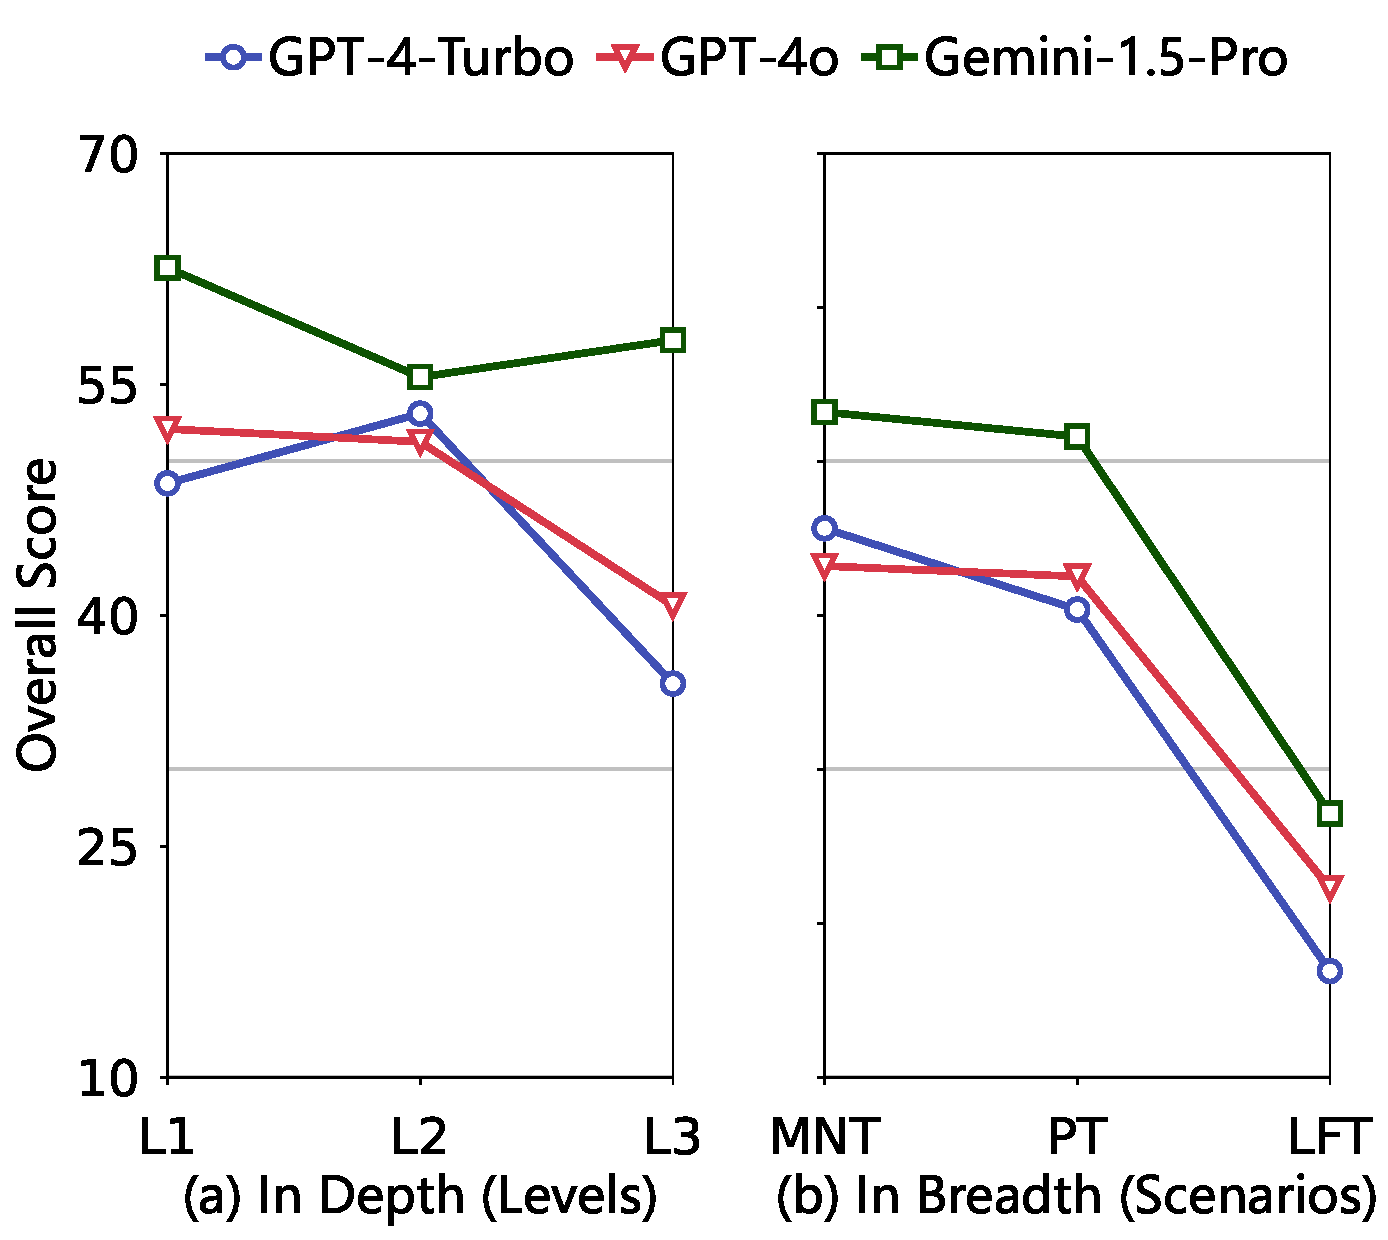
\includegraphics[width=0.48\textwidth]{figures/breadth-depth-yahei0614_new.pdf}
\caption{Performance of top-3 performed models, compared across three scenarios and across levels 1 to 3.}
\label{fig:depth-breadth}
\vspace{-0.5em}
\end{figure}


\subsection{Error Analysis}
\label{ss:error-analysis}
As shown in~\cref{fig:error-analysis}, we conduct a comprehensive error analysis covering various diagnostic tasks and scenarios. 
Based on this analysis, we summarize the identified errors into five types as follows:

\nbf{Non-existent tools.} 
LLMs often predict tools not in the provided tool list, showing a failure to identify available tools and attempting to use non-existent ones.
This error is frequent in Level-2 tasks and LFT scenario of open-weight models but rare in proprietary models.

\nbf{Wrong tools.} 
LLMs use tools not required for the task, indicating a misunderstanding of task requirements or tools' functionality. 
This error is shown in all models, especially in Level-3 tasks and LFT scenarios of proprietary models and in Level-2 tasks of open-weight models.

\begin{figure}[!tp]
\centering
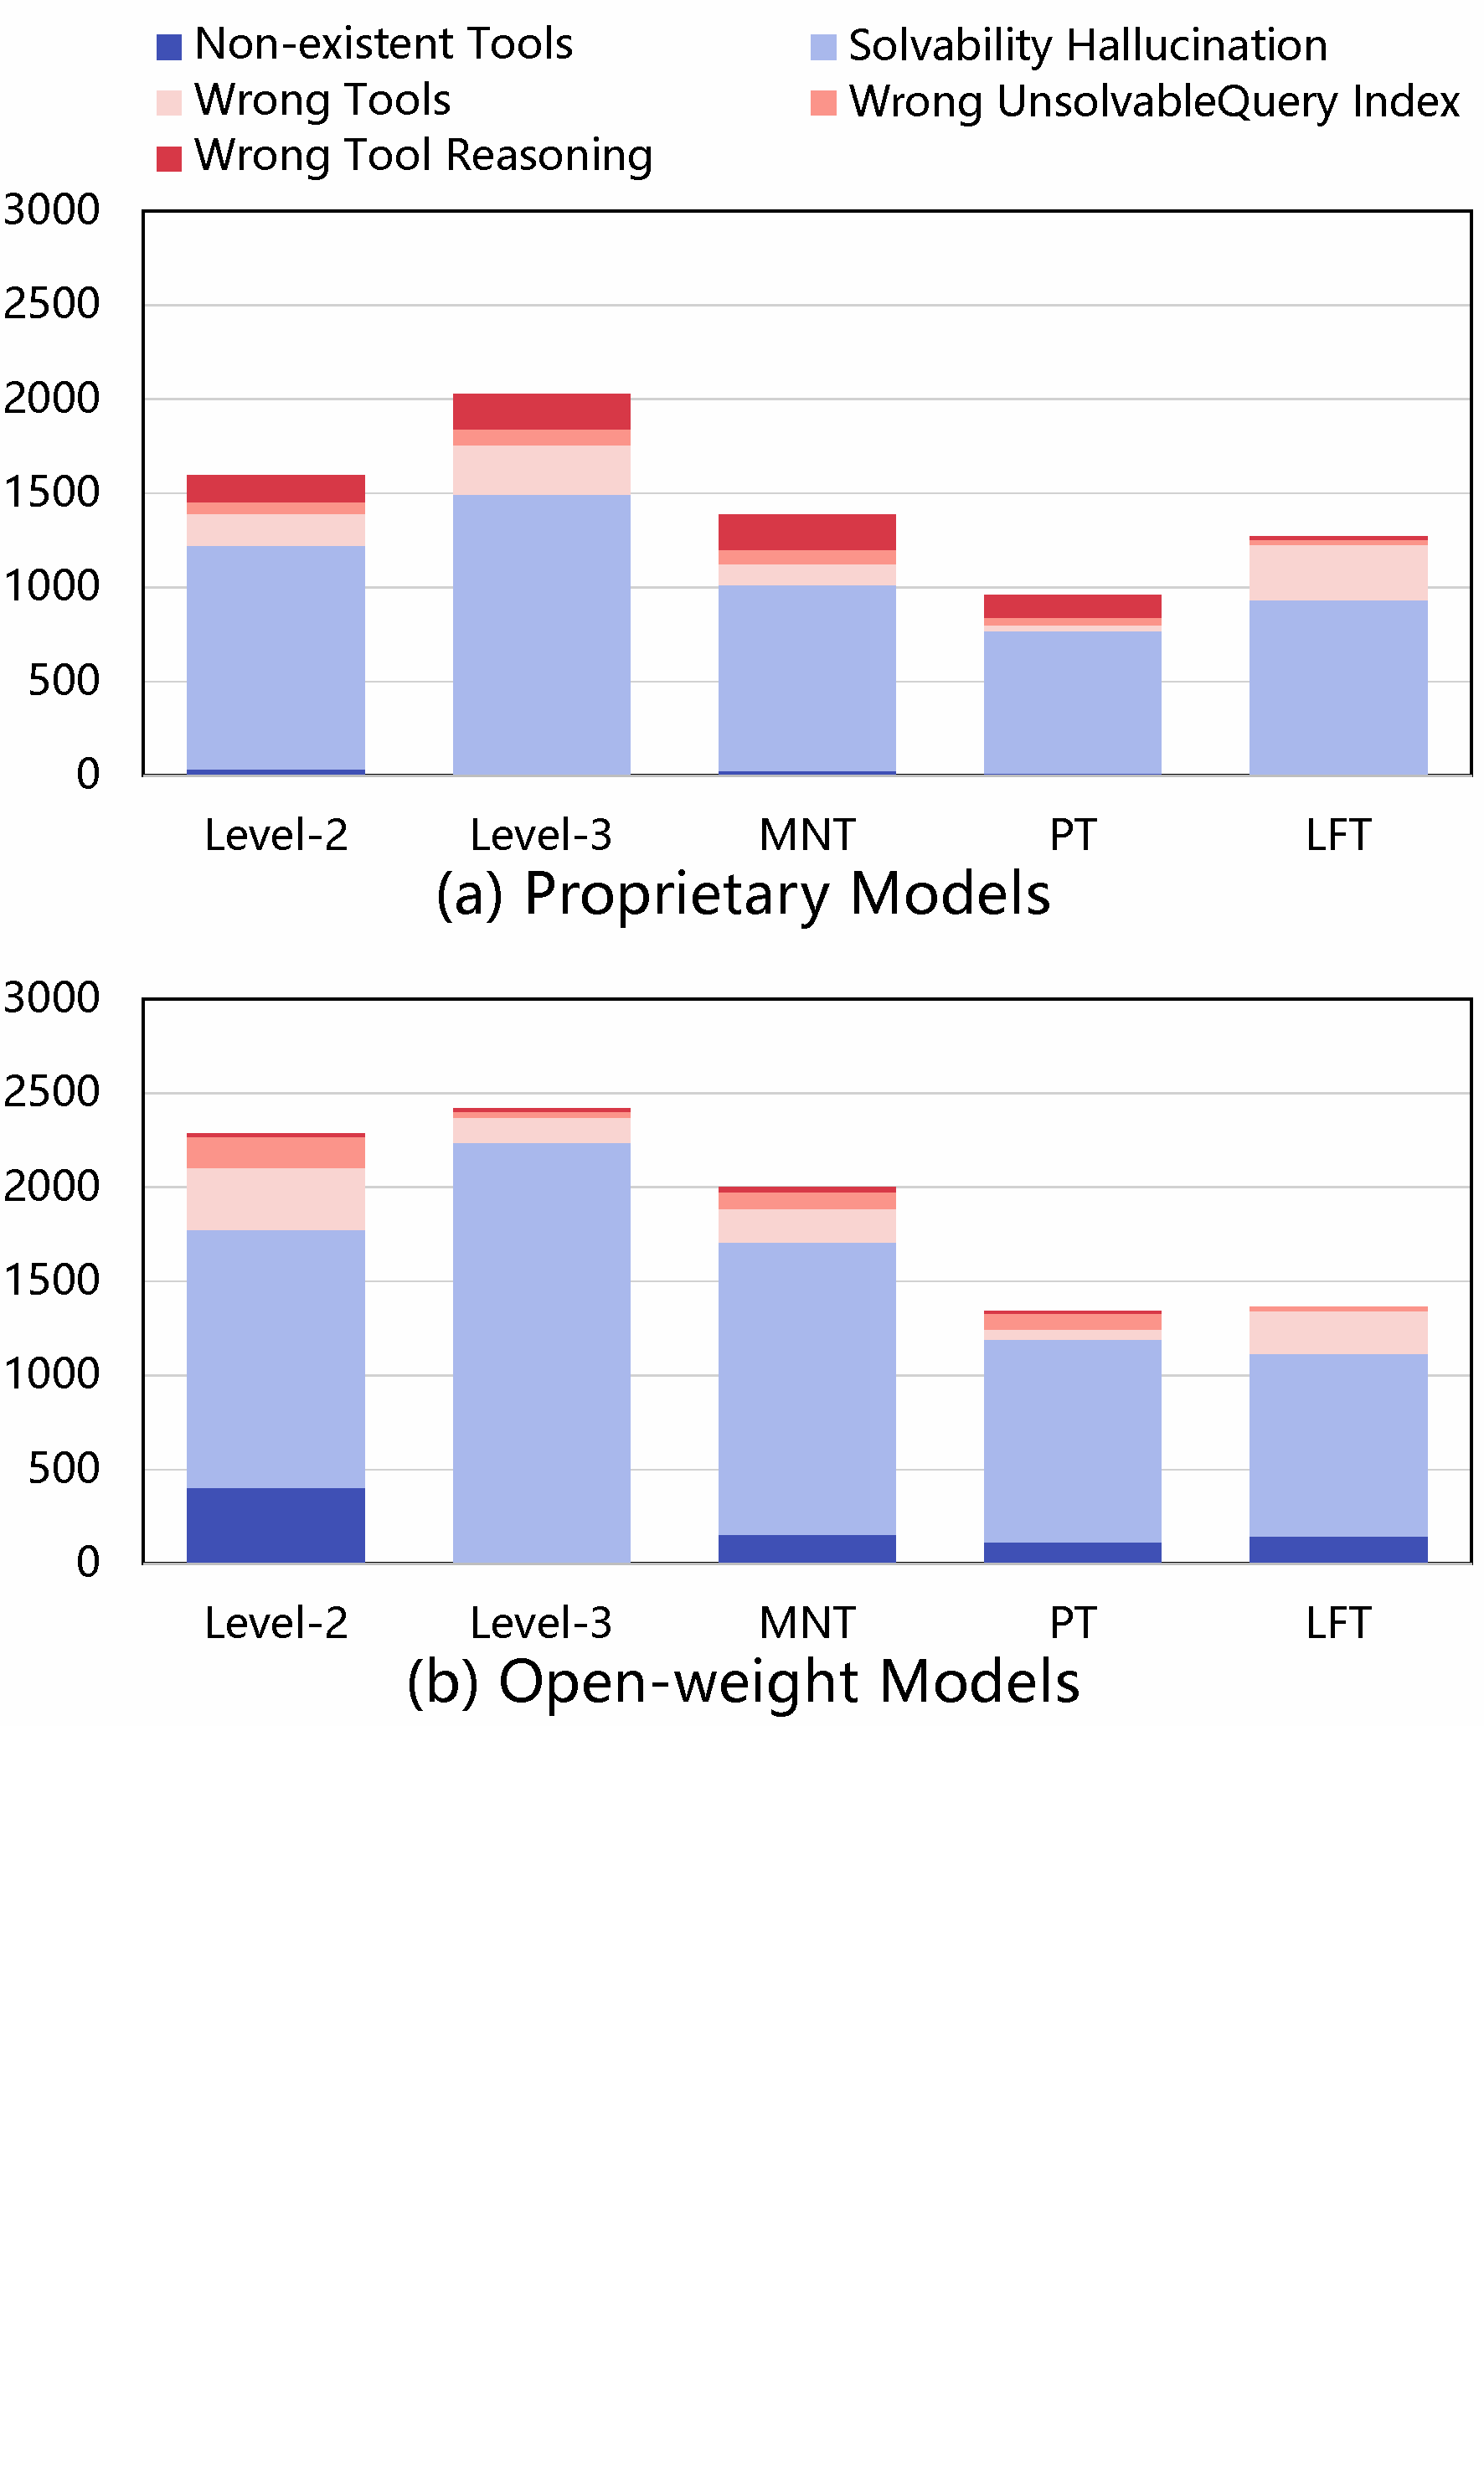
\includegraphics[width=0.48\textwidth]{figures/error-analysis-yahei0614.pdf}
\caption{Error Analysis of proprietary and open-weight models. The Y-axis represents the number of error cases.}
\label{fig:error-analysis}
\vspace{-0.5em}
\end{figure}

\nbf{Solvability hallucination.}
LLMs often fail to identify that a task or subtask is unsolvable, indicating an underestimation of task complexity. 
This is the most common error, particularly in Level-3 tasks.

\nbf{Wrong ``UnsolvableQuery'' index.}
LLMs correctly predict that some tasks or subtasks are unsolvable but misidentify which specific subtasks are unsolvable. 
This error occurs less frequently but is present in all models and stages, indicating a bias in understanding complex tasks.

\nbf{Wrong tool reasoning.}
LLMs do not use tools in the correct sequence, highlighting issues in task logic. 
This error is more prevalent in proprietary models than in open-weight models.  
This is because open-weight models tend to show more ``solvability hallucination'' errors while proprietary models can detect more unsolvable cases. 
Consequently, they cannot perform subsequent tasks, resulting in a smaller number and percentage of errors relative to proprietary models.

Additionally, the outcomes are compared with three akin benchmarks, as delineated in~\cref{append:compare_benchmark}.

\begin{table}[tp]
\setlength{\tabcolsep}{3pt}
\small
\centering
\caption{Results for original solvable and unsolvable tasks. Scores are presented in the format of Solvable Score / Unsolvable Score.}
% \vspace{1em}
\resizebox{0.48\textwidth}{!}{
\begin{tabular}{l|c|c|c|c}
\toprule
\multicolumn{1}{c|}{Model} & L1 & L2 & L3 & Overall \\
\midrule
\multicolumn{5}{c}{\textit{Proprietary}} \\
\midrule
\multirow{1}{*}{Gemini-1.0-Pro} & 98.9 / 13.1 & 83.1 / 10.0 & 84.3 / 29.5 & 88.7 / 20.6 \\
\midrule
\multirow{1}{*}{GPT-4o} & 95.4 / 52.3 & 88.3 / 53.9 & 83.2 / 21.0 & 89.0 / 37.0 \\
\midrule
\multicolumn{5}{c}{\textit{Open-weight}} \\
\midrule
\multirow{1}{*}{Llama-3-8B} & 93.7 / 20.6 & 74.9 / 3.6 & 64.4 / 4.2 & 77.6 / 8.1 \\
\midrule
\multirow{1}{*}{Llama-3-70B} & 100.0 / 28.6 & 86.2 / 23.1 & 66.8 / 3.3 & 84.3 / 14.6 \\
\midrule
\multicolumn{5}{c}{\textit{Performance Ratio of Open-weight to Proprietary Models (\%)}} \\
\midrule
- & 99.7 / 75.2 & 94.0 / 41.8 & 78.3 / 14.9 & 91.1 / 39.4 \\
\midrule
\bottomrule
\end{tabular}}
% \vspace{-1.0em}
\label{tab:s-vs-uns}
\end{table}

\subsection{Solvable Tasks Versus Corresponding Unsolvable Tasks}
\label{append:solvable_test}

During our iterative annotation process described in~\cref{ss:data-curation}, we emphasize fairness and objectivity in data curation and implement thorough manual curation and refinement throughout the synthesis process.
To evaluate potential biases introduced by the data generation process using proprietary models, we conduct a comprehensive comparison across proprietary and open-weight models on generated solvable problems and their corresponding unsolvable counterparts, which is human-crafted.

As shown in~\cref{tab:s-vs-uns}, there are minimal performance discrepancies between LLMs under solvable tasks. 
Despite the inherent capability gaps between open-weight and proprietary models, open-weight models achieve $91.1\%$ of the performance of proprietary models.

This indicates that biases in data generated by proprietary models are effectively minimized following human intervention.
However, the performance disparity becomes substantially larger when assessing unsolvable tasks.
Open-weight models can only achieve $39.4\%$ of the performance when compared to proprietary models.
This discrepancy is particularly noteworthy given that recent benchmarks assume a strong premise: users will provide a complete list of tools, each accompanied by detailed explanations~\cite{DBLP:journals/corr/abs-2401-13178@agentboard,DBLP:journals/corr/abs-2307-16789@toolbench,DBLP:conf/nips/ZhuangYWSZ23@toolqa,DBLP:journals/corr/abs-2308-03688@agentbench}. 
This highlights the importance of unsolvable tests in comparing model performance within tool-using scenarios.

\section{Conclusions}
\label{conclusion}

This paper introduces the \benchname benchmark for diagnosing hallucinations in tool-augmented LLMs.
Specifically, we evaluate hallucination from the perspective of depth (multi-level evaluation framework) and breadth (three scenarios to induce hallucinations).
Our results indicate that LLMs are prone to hallucinations even in straightforward tool-using tasks under unsolvable conditions. 
The impact of the quantity and quality of the training data, response strategy, and long-context reasoning consistency on the performance should be addressed.
Error analysis reveals that LLMs primarily struggle with solvability hallucination, characterized by their inability to comprehend user queries and accurately interpret the tools and their functions. 
This often leads these models to mistakenly conclude that they can solve tasks.
Our \benchname marks a pivotal advancement in diagnosing hallucinations, providing resources for exploring the real-world performance of tool-augmented LLMs.

\section*{Limitations}

Our analysis may need to be more comprehensive as it does not include a broader range of open-source LLMs, such as cross-linguistic models. 
The focus is solely on dense architectures and mixture-of-experts, considering only these structures and varying parameter sizes known to influence performance.
Additionally, the limited scope of only seven models could introduce bias into our findings.  
To mitigate these limitations, \textbf{we will open-source all data and methods} to assist users and developers by simplifying the evaluation process.

In our tool design, we only reference practices similar to the methods in MetaTool~\cite{DBLP:journals/corr/abs-2310-03128@metatool}, where only tool names are provided without additional details such as API parameters. 
This approach could lead to discrepancies between our evaluation benchmarks and real-world applications. 
Fortunately, as is inherent to its design, our framework is scalable and, therefore, capable of incorporating a broader range of tools, including those that use APIs with parameters.
This flexibility allows the community to effortlessly swap tools based on our guidelines and conduct more comprehensive analyses of model performance.

\section*{Ethical Considerations}

As our data is derived from synthetic sources, it is possible that certain ethical biases may be present. 
Manual interventions have been incorporated into the filtering process to mitigate potential ethical bias. 
However, it should be acknowledged that this does not guarantee the complete elimination of these biases. 
Furthermore, since all the members of our annotation team are from the same country, there may be an inherent regional characterization that hinders the effective filtering of biases prevalent in other regions.
Consequently, it is recommended that additional bias mitigation strategies be employed, such as the ethical alignment techniques~\cite{DBLP:conf/sigir-ap/YuWZZYS23@ethical}, diverse annotation panel~\cite{shi2024chartmimic} or custom rules, before utilizing the aforementioned data.

\bibliography{toolbh}

\clearpage
\appendix
\section*{Appendix}

\section{Details of Benchmark Curation}
\label{append:details-benchmark}

\subsection{Design Considerations of the Multi-level Evaluation Methods}
\label{append:necessity-multi-level}

In this section, we present our design considerations from the perspective of depth in hallucinations~\cref{ss:multi-level-evaluation}. 

In \textbf{Level-1 (Solvability Detection)}, the task is to determine whether a given user query can be solved using the available tools from a macro perspective. 
It effectively filters out tasks that require further analysis, identifying those deemed unsolvable from a macro-level judgment, and allows the system to focus on tasks that might have been incorrectly evaluated at this level.

In \textbf{Level-2 (Solution Planning)}, the purpose is to refine the solution by determining at which step the task becomes problematic.

Once Level-1 has been evaluated from a macro perspective, a more detailed analysis will be conducted to identify the specific steps involved in hallucination during the task.
Consequently, the task requirement is divided into several sub-goals from the perspective of task decomposition. 
With this setup, a detailed breakdown of the steps required to solve the task is provided, enabling the identification of which steps involve the correct use of the tool and which are incorrect. 
This lays the groundwork for a more in-depth analysis.

In \textbf{Level-3 (Missing-Tool Analysis)}, when a sub-goal is identified as unsolvable in Level-2, understanding why the current tools fail to achieve this sub-goal is crucial.
Therefore, the task requires the model to describe the functions of the missing tools, thus revealing specific deficiencies.
The analysis of missing tools allows for further analysis of the model's understanding of tool characteristics, such as tool functionality. 
Furthermore, such an analysis can benefit real-world scenarios, assisting developers in refining the toolset. 

In summary, we present a hierarchical approach to diagnosing model hallucinations based on the model's progressive understanding of user queries and available toolsets. Our methodology comprises three distinct levels of analysis:
At Level-1, the model conducts a marco assessment of the information provided by the user query.
Proceeding to Level-2, the model decomposes the overarching objective into multiple sub-goals and attempts to address them using provided tools.
Finally, at Level-3, the model performs an in-depth analysis of each tool's characteristics, such as functionality, concerning each sub-goal.
This three-tiered approach offers a perspective on hallucination analysis that spans different depths of comprehension. 
It enables a comprehensive examination of unsolvable tasks involving tool use, progressing from macro to micro levels and general to specific details.
This analytical framework facilitates a profound understanding of hallucinations in LLMs and potentially provides a valuable direction for future research aimed at mitigating the occurrence of such phenomena.


\subsection{Filtering Criteria}
\label{append:filter-criteria}

In~\cref{ss:data-curation}, we mentioned several filtering methods in~\textbf{(3) Filtering}. 
We define the corresponding criteria as follow.

\nbf{Semantic similarity check.} 
We employ embedding models \texttt{all-MiniLM-L6-v2} and compute the semantic similarity between each synthetic sample and the seed sample. 
We exclude samples with task similarity and tool similarity scores greater than $0.8$ to avoid redundancy and ensure dataset diversity.
    
\nbf{Filtering with python code.} 
In the subtasks except for ``Single-step'', a simple matching algorithm is employed to eliminate ambiguous tasks and retain only samples with clearly itemized task requirements. 
Concurrently, it is verified that all tools mentioned in the ground truth solutions are included in the provided list of tools. 
Furthermore, responses are tailored to align with the specific requirements of different subtasks based on their characteristics. For instance, the ``Iterative'' task necessitates repeated consecutive use of the same tool.
    
\nbf{Manual review process.}
Samples that are unclear in expression, contain logical fallacies, or have poor argumentation between the sub-goal description and the tool used are removed. 
Furthermore, potential ethical biases, including but not limited to gender and racial biases, are eliminated from the dataset.

\subsection{Generation Prompts}
\label{append:generation_prompt}

In~\cref{benchmark:hallu_scena}, we provide a comprehensive description of the hallucination-inducing tasks within our benchmark. 
We designed corresponding prompts based on the characteristics of subtasks in various scenarios. 
The specific content of these prompts can be found from~\cref{fig:single-step-prompt} to~\cref{fig:best-prompt}.


\subsection{Evaluation Prompts}

In~\cref{ss:multi-level-evaluation}, we present a detailed analysis of the hallucination phenomenon from the perspective of depth. we set the temperature to $0.0$ and maintained other default settings~\cite{shi2024thorough}.
Specially, we conduct a series of processing operations on the model output, as outlined below.

The different levels of evaluation prompts are manually constructed by wrapping both the task description section and the provided tools section in particular XML elements. 
The task description is marked with the tags <task> and </task> and the provided tools with the tags <provided\_tools> and </provided\_tools>, respectively. Furthermore, we require that LLMs use the tags <answer> and </answer> to enclose the answer part. 
We require that redundancies be avoided in the output to minimize the tendency of LLMs to produce long answers or detailed explanations.

We provided a corresponding prompt and example for each level of the task from~\cref{fig:level-1_prompt} to~\cref{fig:level-3_prompt}. 
In Level-1, we focus on determining the solvability of the task; Level-2 requires the model to split and prioritize subtasks based on available tools; Level-3 further demands the model to analyze tool usage and identify missing tool functionalities. 
These prompts are designed to progressively increase task complexity, comprehensively assessing the hallucination state within tool-augmented LLM scenarios.

\subsection{License}

Our benchmark data and code are released under the MIT License, which is detailed in~\url{https://opensource.org/licenses/MIT}.

\section{Comparisons with Existing Benchmarks}
\label{append:compare_benchmark}

In this section, we present a comprehensive comparison with existing, widely-used tool-based benchmarks, providing a detailed analysis of our findings.

Our benchmark presents a greater challenge compared to previous tool-based benchmarks.
In the AgentBoard for tool-related Tool-Query task\cite{DBLP:journals/corr/abs-2401-13178@agentboard}, $8$ out of $13$ evaluated models scored between $60.0$ and $85.1$ points.
However, the performance disparity among these models on our benchmark is notably significant.
For instance, the performance difference between GPT-4 and GPT-3.5-Turbo is $18.4\%$.
Similarly, StableToolBench~\cite{DBLP:journals/corr/abs-2403-07714@stabletoolbench} showed a modest disparity among top-performing models, with a difference of $11.3\%$ between GPT-3.5 and GPT-4.
This gap widens to $57.7\%$ on our \benchname benchmark.

This reflects our multi-level assessment's ability to discern nuanced differences in LLM capabilities, providing a comprehensive evaluation of LLMs' proficiency across similar tasks.

Furthermore, our benchmark enhances the error analysis granularity compared to MetaTool’s reliability task.
MetaTool~\cite{DBLP:journals/corr/abs-2310-03128@metatool} conducted reliability tests requiring the output of the correct tool or ``None'' if no appropriate tool exists, which is similar to our Level-1 task.
Their tasks generally involved a single sentence with a single requirement and only required the output of one tool.
Conversely, our benchmark introduces complex, multi-layered scenarios that pose a broader range of challenges.
For example, while GPT-3.5 achieved a score of $50.35$ on MetaTool’s reliability task, it managed only an average score of $18$ on our Level-1 task.

Moreover, MetaTool did not fully explore the diversity of scenarios that models may encounter, leading to their conclusion that LLMs often produce irrelevant tool responses (corresponding to our ``Wrong Tools'' error type). 
In our benchmark, through analysis at multi-level tasks, reveals that while ``Wrong Tools'' is a common error type for these models, the core issue lies in their inability to discern task solvability, manifesting as ``Solvability Hallucination''.

Furthermore, our benchmark introduces a more sophisticated multi-level evaluation and incorporates a wider array of task scenarios, enabling a more nuanced analysis of hallucinations. 
These enhancements allow for a detailed investigation into the reasons behind these inaccuracies, as discussed in~\cref{ss:error-analysis}. 
This comprehensive approach aids the community in gaining a deeper understanding of why such hallucinations occur, improving model evaluation methodologies and addressing gaps in current benchmarking practices.


\section{Details of Experimental Setting}

\subsection{Version for Tested Proprietary Models}
\label{append:experimental-setting}
 
We provide detailed versions of all tested proprietary models to ensure the reproducibility of results.
\begin{itemize}
\setlength{\itemsep}{1pt}
\setlength{\parskip}{2pt}
\setlength{\parsep}{0pt}
\item Gemini-1.0-Pro: \texttt{models/gemini-1.0-pro}, Version: gemini-1.0-pro-002
\item Gemini-1.5-Pro: \texttt{models/gemini-1.5-pro}, Version: gemini-1.5-pro-preview-0514
\item GPT-3.5-Turbo: \texttt{gpt-3.5-turbo-0125}
\item GPT-4-Turbo: \texttt{gpt-4-turbo-2024-04-09}
\item GPT-4-1106: \texttt{gpt-4-1106-preview}
\item GPT-4-0613: \texttt{gpt-4-0613}
\item GPT-4o: \texttt{gpt-4o-2024-05-13}
\end{itemize}

\subsection{Different Embedding Models in Level-3 Matching Score}

In Level-3, the cosine similarity between tools is calculated using embedding models.
Therefore, we test the L3-MS scores of these models to assess the impact of different embedding models on MS score computation.
As presented in~\cref{tab:embedding_gap}, we consider the proprietary embedding model~\texttt{text-embedding-004}~\footnote{\url{https://ai.google.dev/gemini-api/docs/models/gemini\#text-embedding-and-embedding}} (referred to as Gemini) and the open-weight embedding model~\texttt{all-MiniLM-L6-v2} (referred to as~MiniLM).
The details of the two embedding models are listed.

\begin{itemize}
\setlength{\itemsep}{1pt}
\setlength{\parskip}{2pt}
\setlength{\parsep}{0pt}
\item\texttt{text-embedding-004}:
\begin{itemize}
    \item Input: Text
    \item Output: Text embeddings
    \item Input token limit: $2,048$
    \item Output dimension size: $768$
    \item Latest update: April 2024
\end{itemize}

\item \texttt{all-MiniLM-L6-v2}:
\begin{itemize}
    \item Input: Text
    \item Output: Text embeddings
    \item Input token limit: $512$
    \item Output dimension size: $384$
\end{itemize}
\end{itemize}

In result, the negligible variance in the L3-MS scores across different embedding models presents the robustness of our task and metric frameworks.
Consequently, we select the~\texttt{all-MiniLM-L6-v2} model as default embedding model.


\section{Additional Experiments and Result Analysis}

\begin{table}[tp]
\small
\centering
\caption{Results for Level-3 Match Score using different embedding models.}
\begin{tabular}{l|c|ccc}
\toprule
\multicolumn{2}{l|}{Model} & \multicolumn{1}{c|}{MNT} & \multicolumn{1}{c|}{PT} &  \multicolumn{1}{c}{LFT}  \\
\midrule
\multicolumn{5}{c}{\textit{Proprietary}} \\
\midrule
GPT-4o & \makecell{Gemini \\ MiniLM} & 
\makecell{26.5 \\ 24.8} & \makecell{37.2 \\ 33.2} & \makecell{5.9 \\ 4.4} \\
\midrule
Gemini-1.0-pro & \makecell{Gemini \\ MiniLM} & 
\makecell{38.7 \\ 35.3} & \makecell{43.4 \\ 38.9} & \makecell{2.1 \\ 1.8} \\
\midrule
GPT-3.5-Turbo & \makecell{Gemini \\ MiniLM} & 
\makecell{21.9 \\ 21.0} & \makecell{15.2 \\ 14.0} & \makecell{0.7 \\ 0.2} \\
\midrule
\multicolumn{5}{c}{\textit{Open-weight}} \\
\midrule
Llama-3-70B & \makecell{Gemini \\ MiniLM} & 
\makecell{4.8 \\ 4.9} & \makecell{5.2 \\ 4.3} & \makecell{0.0 \\ 0.0} \\
\midrule
Llama-3-8B & \makecell{Gemini \\ MiniLM} & 
\makecell{6.6 \\ 6.1} & \makecell{3.9 \\ 2.9} & \makecell{0.7 \\ 0.7} \\
\midrule
Average Gap & - & 
1.3 & 2.3 & 0.5 \\
\bottomrule
\end{tabular}
\label{tab:embedding_gap}
\end{table}

\subsection{How Does Response Length Impact Performance?}
\label{append:pred_length}

\begin{figure*}[!tp]
\centering
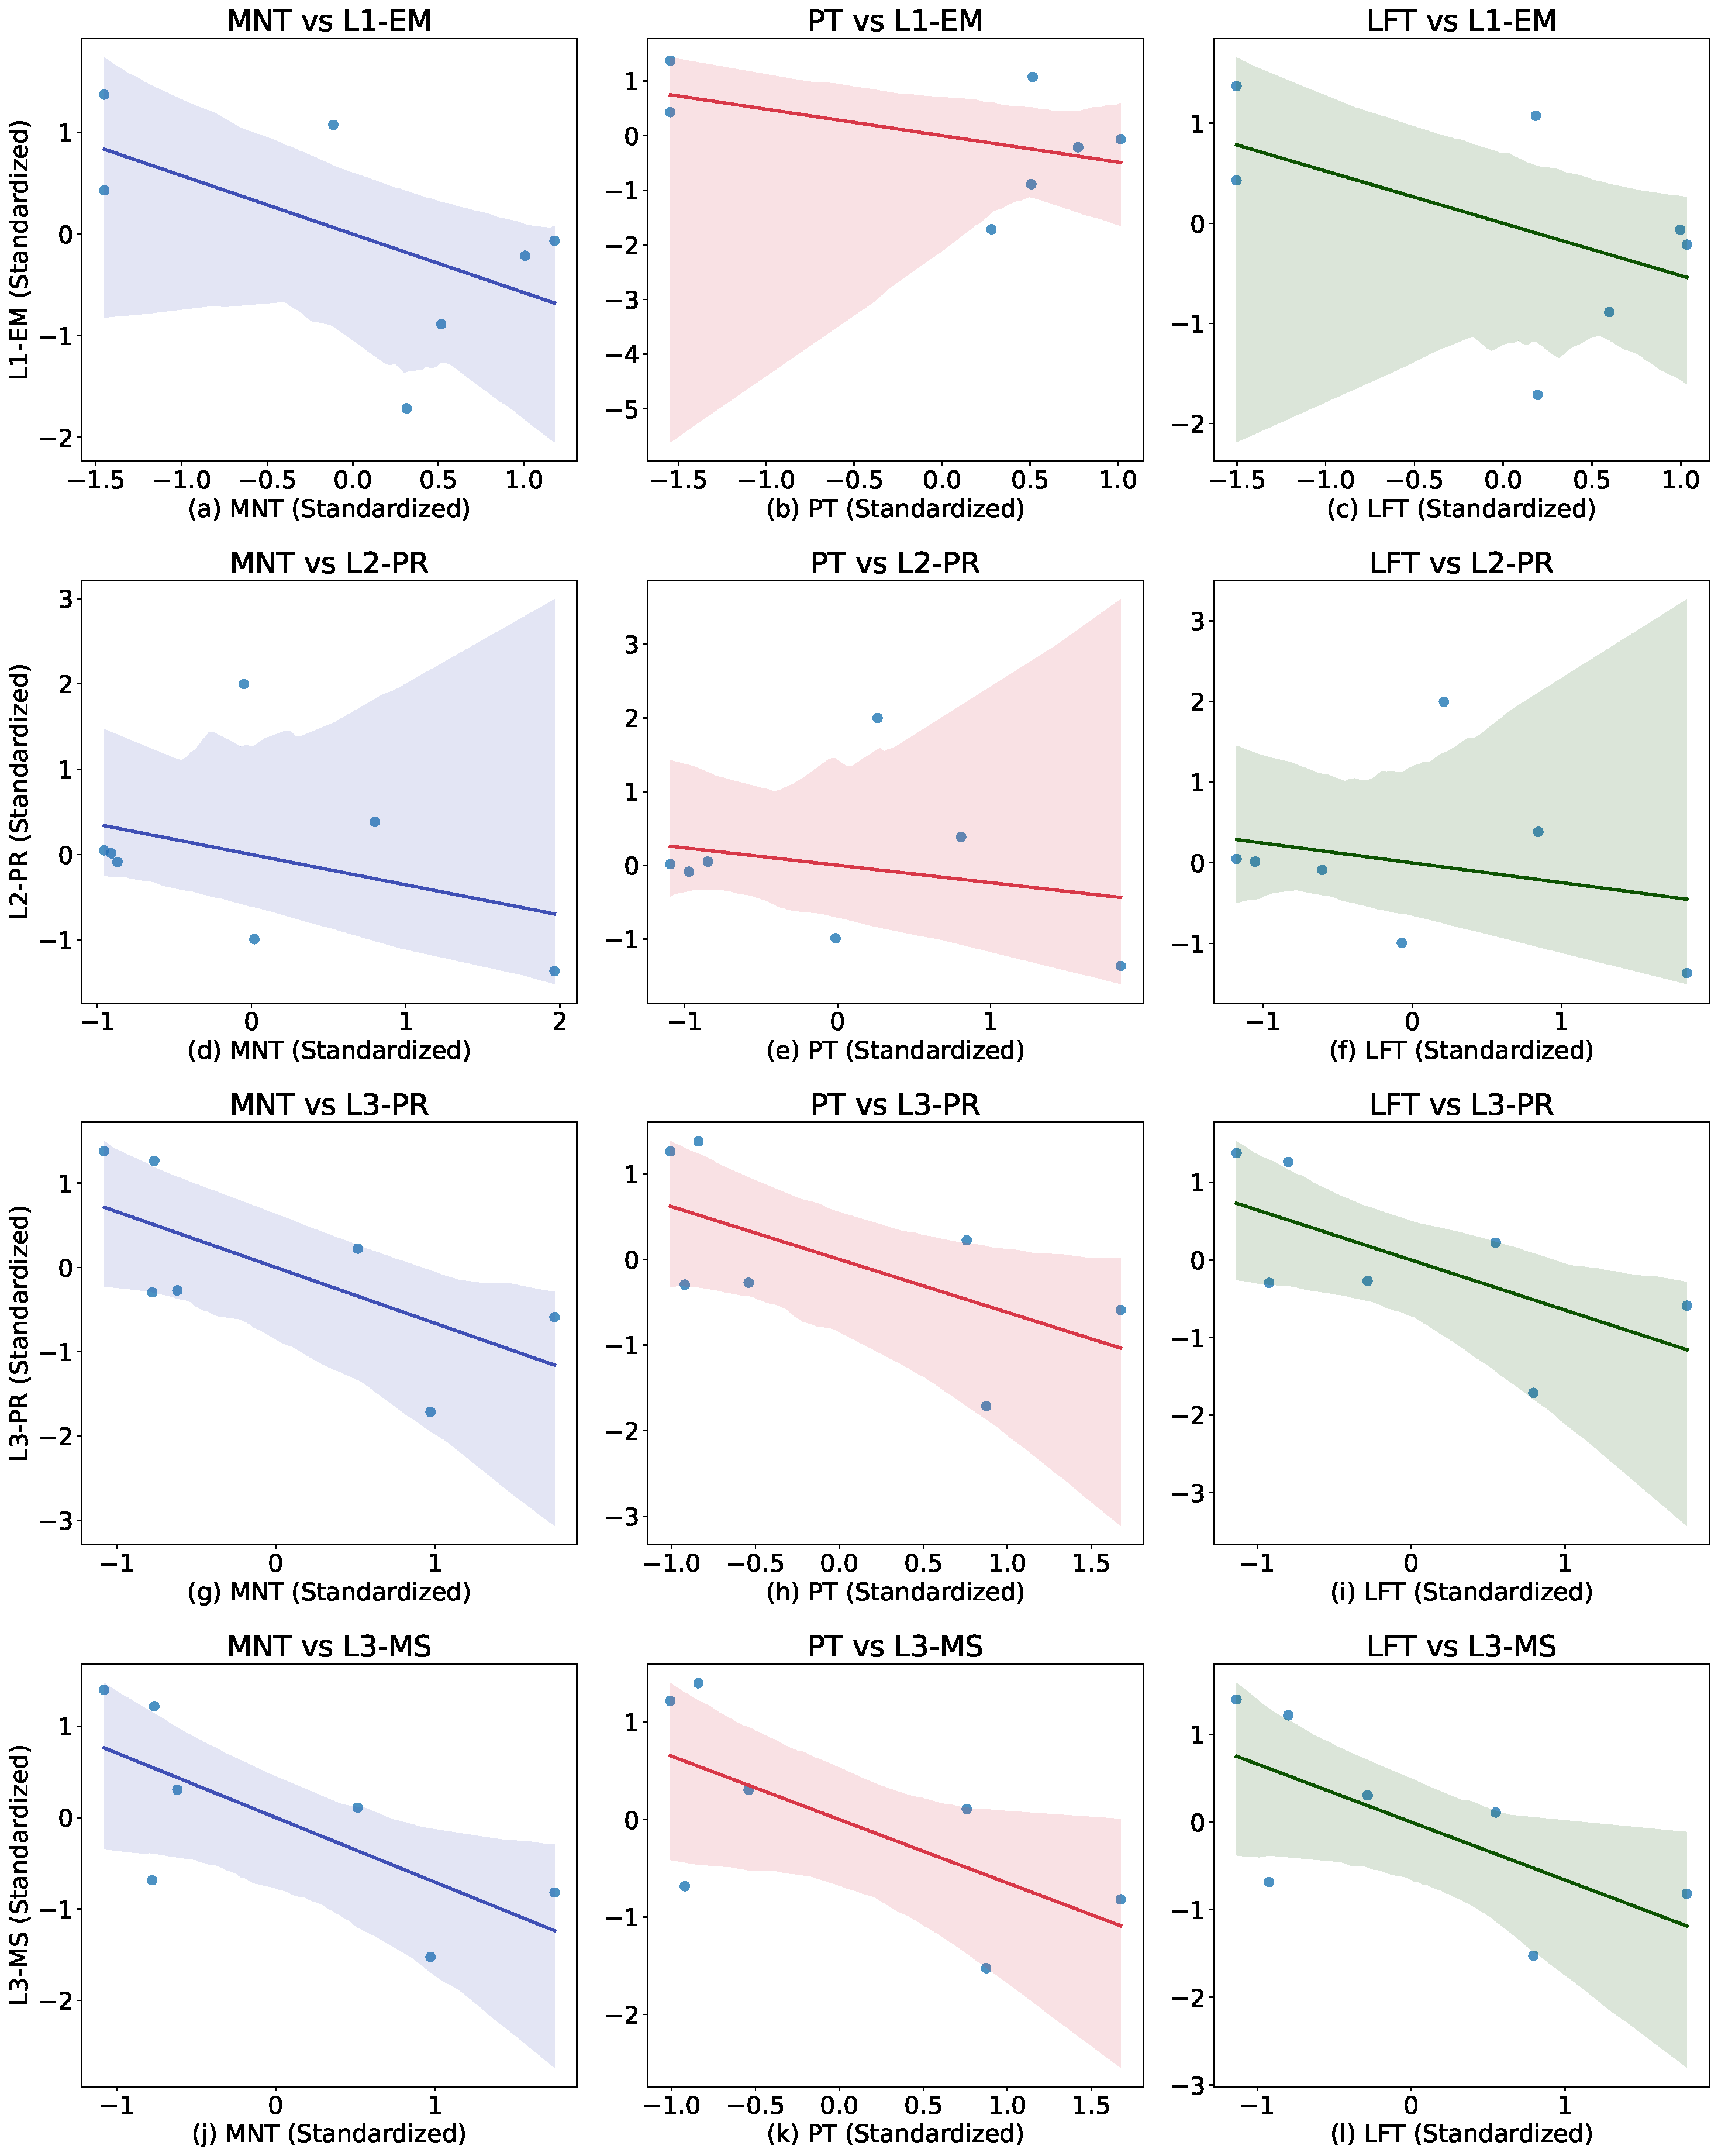
\includegraphics[width=0.98\textwidth]{figures/OS_models_all_comparisons.pdf}
\caption{Standardized relationships between response length and performance indicators for open-weight LLMs across three tool availability scenarios. 
Performance indicators: L1-EM (Level-1 Exact Match), L2-PR (Level-2 Progress Rate), L3-PR (Level-3 Progress Rate), and L3-MS (Level-3 Matching Score). 
Scenarios: MNT (Missing Necessary Tools), PT (Potential Tools), and LFT (Limited Functionality Tools). 
Each row depicts a specific performance indicator, while columns represent different scenarios.}
\label{fig:length-vs-perf-os}
\end{figure*}

\begin{figure*}[!tp]
\centering
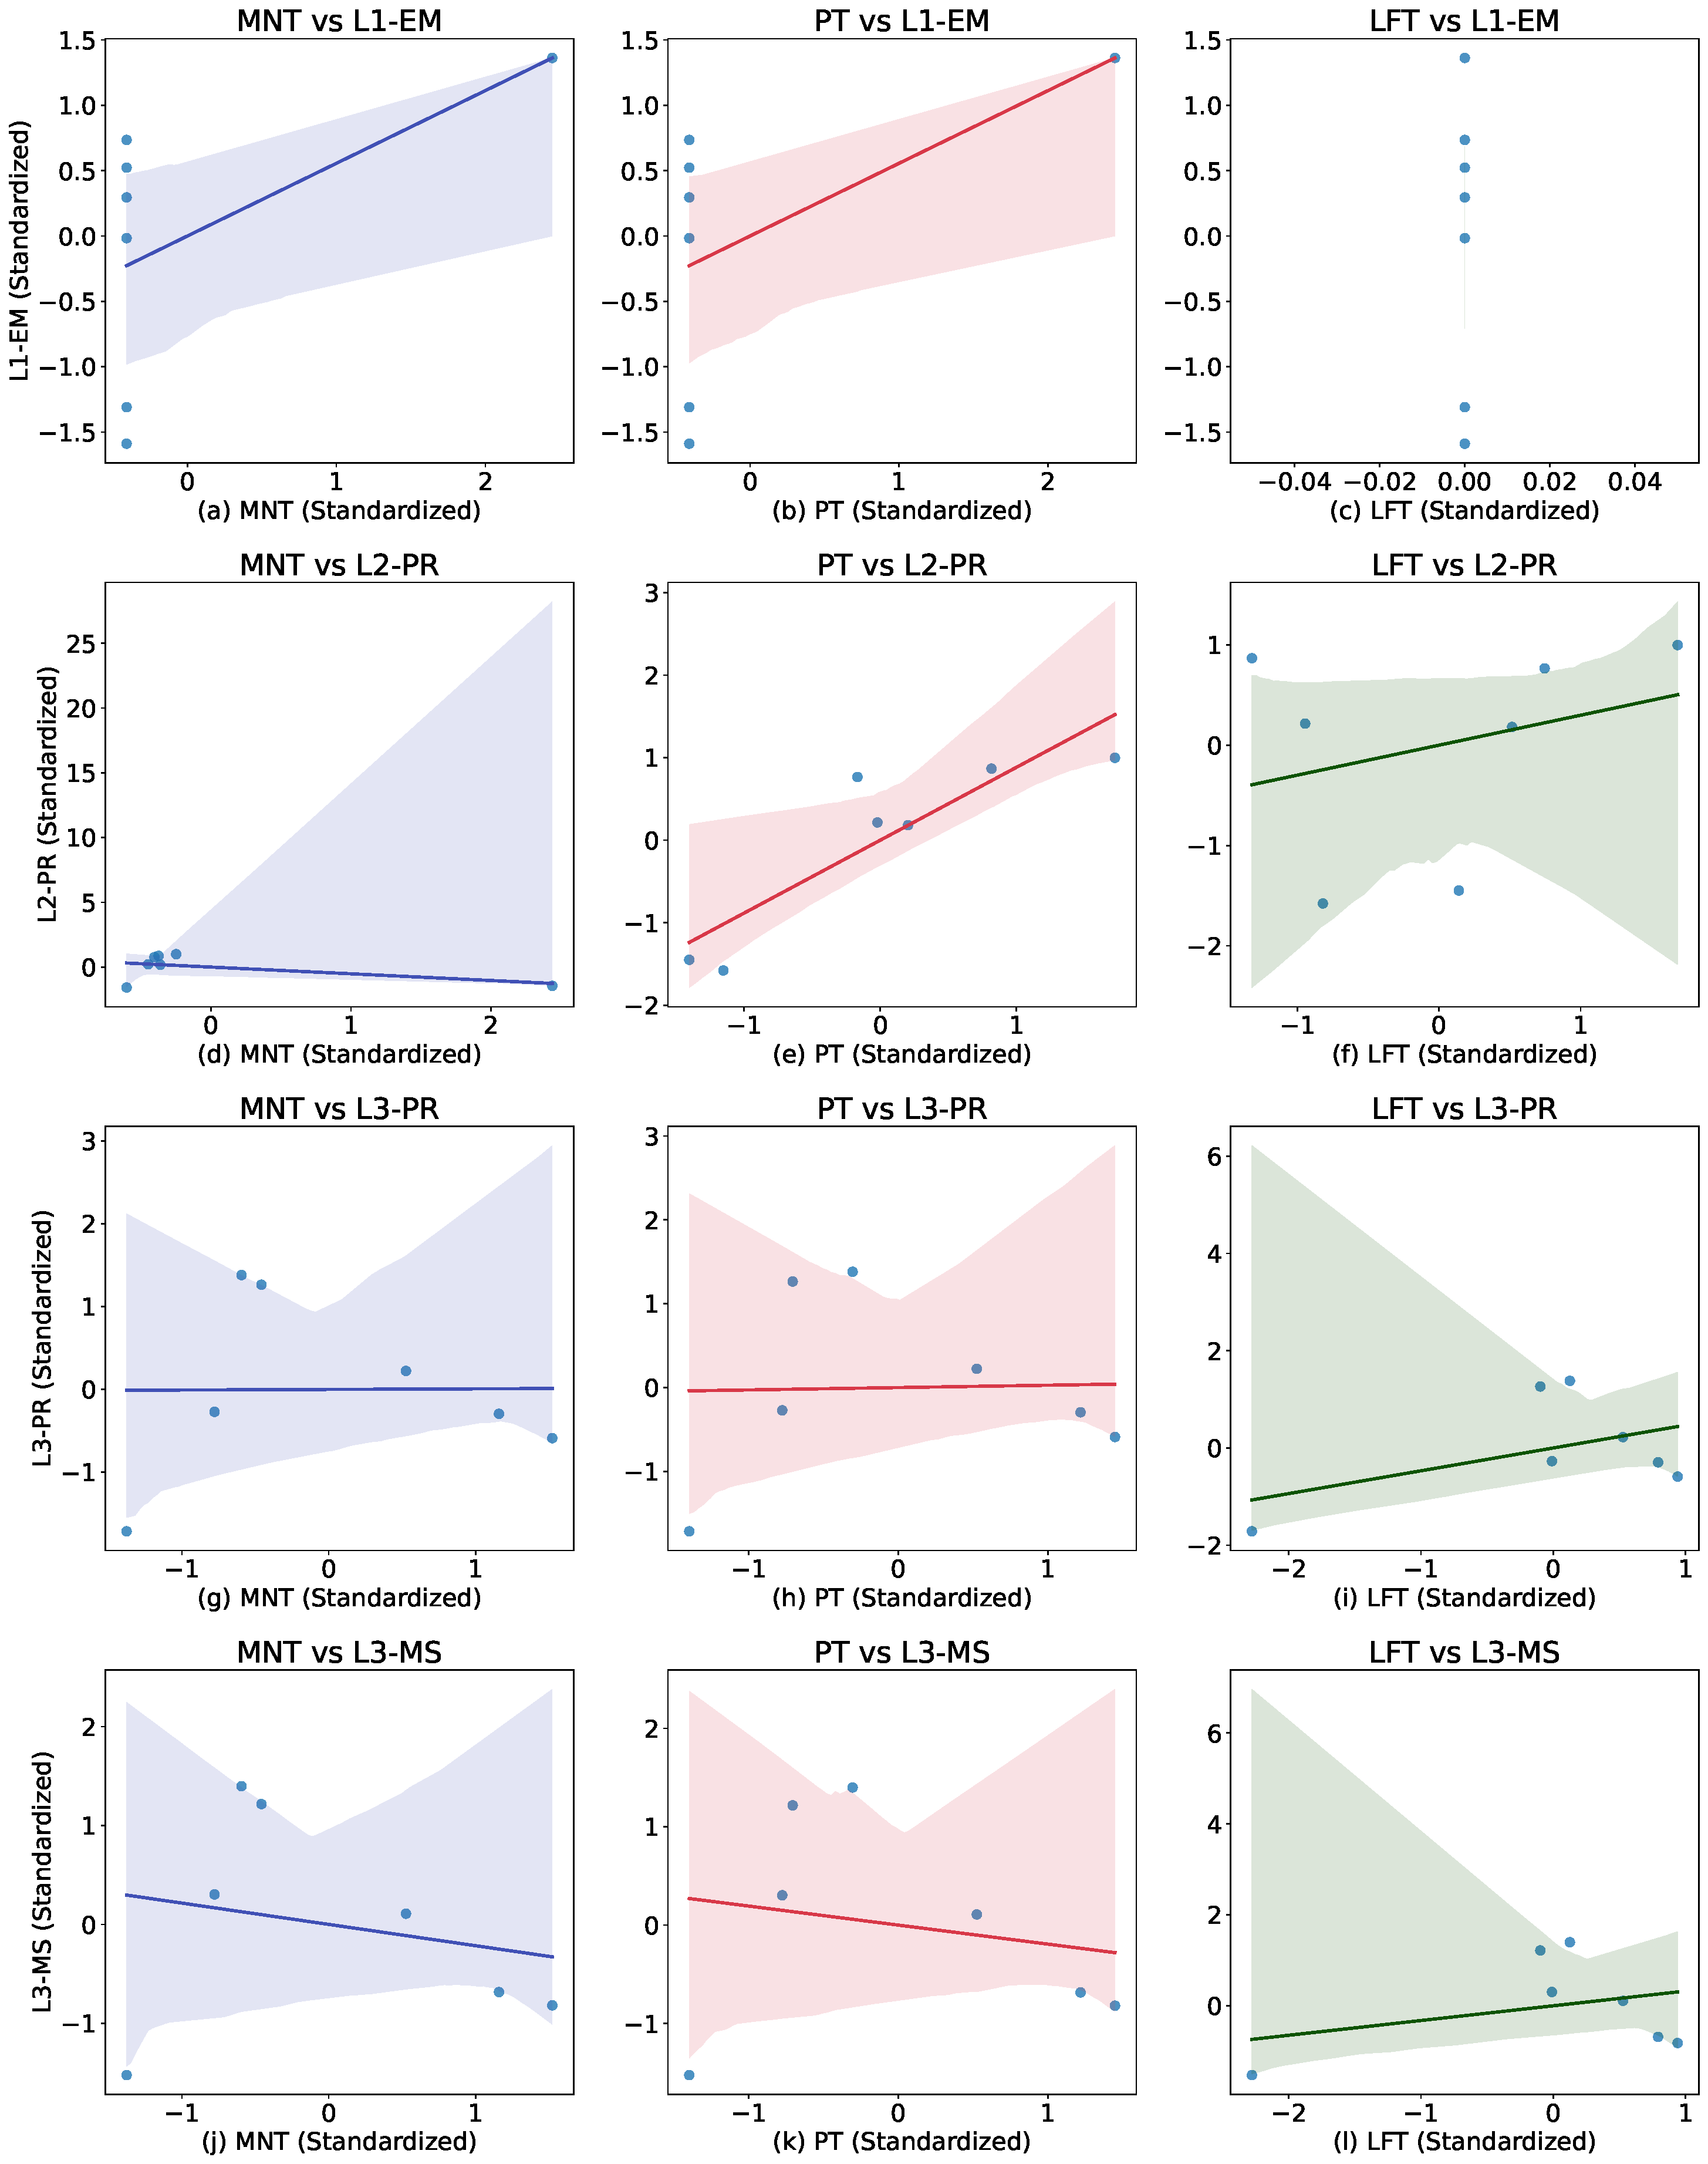
\includegraphics[width=0.98\textwidth]{figures/CS_models_all_comparisons.pdf}
\caption{Standardized relationships between response length and performance indicators for proprietary LLMs across three tool availability scenarios. 
Performance indicators: L1-EM (Level-1 Exact Match), L2-PR (Level-2 Progress Rate), L3-PR (Level-3 Progress Rate), and L3-MS (Level-3 Matching Score). 
Scenarios: MNT (Missing Necessary Tools), PT (Potential Tools), and LFT (Limited Functionality Tools). 
Each row depicts a specific performance indicator, while columns represent different scenarios.}
\label{fig:length-vs-perf-cs}
\end{figure*}

We systematically compare the relationship between response length and performance across all levels and scenarios. 
As shown in~\cref{fig:length-vs-perf-os} for open-weight models and~\cref{fig:length-vs-perf-cs} for the proprietary models, we collect data points ($X$, $Y$), representing response lengths ($X$) and corresponding performance ($Y$) at different levels.
After standardizing the data, we created scatter plots with regression lines to depict the trends between response length and scores visually. 
This approach allows us to intuitively observe positive, negative, or no correlation between length and performance scores.


\subsubsection{Open-weight Models: Negative Correlation with Response Length}

For the open-weight models, the regression lines for all levels (L1 to L3) and all scenarios (MNT, PT, LFT) trend downward. 
This indicates that the overall performance scores tend to decrease as the response length increases.

We observe that open-weight models often generate longer responses for task planning, which may include excessive redundant information and unnecessary conversational elements. 
This phenomenon might obscure critical steps and tool choices with irrelevant information, negatively impacting task accuracy and overall scores.
One reason is that, influenced by the format of training data and preferred response strategy, the generation of responses with conversational characteristics may be prioritized, resulting in responses filled with irrelevant explanations and extensions. 
This tendency towards over-explanation and verbosity generally leads to poorer performance under task-oriented evaluation criteria. 
To optimize this, one possible solution is to introduce more task-oriented examples during training to reduce the emphasis on generating conversational features and encourage the generation of concise, relevant task plans. 
Moreover, it is imperative to enhance the capacity of these models to maintain information consistency and logical coherence in complex tasks involving long-text.

\subsubsection{Proprietary Models: Positive Correlation with Response Length}

For proprietary models, all scenarios and levels exhibit regression lines that are either flat or trend upward, with the exception of a slight downward trend observed in L3-MS for MNT and PT. 
This suggests that, in contrast to open-weight models, longer response lengths in proprietary models are associated with higher performance scores.
In addition, proprietary models demonstrate superior performance in adhering to the task instructions provided. As illustrated in~\cref{fig:length-vs-perf-cs} (c), all proprietary models have the same token length, suggesting that they are all capable of following the instructions and avoiding the generation of redundant outputs.

Proprietary models exhibit an enhanced aptitude for maintaining contextual consistency in extended responses, thereby furnishing comprehensive and pertinent information. 
This capability enables these models to perform well in complex tasks and long-text reasoning, where longer responses improve task execution coherence and accuracy, rather than introducing redundancy.
Proprietary models appear to prioritize long-text reasoning and contextual processing during the data designing and model training phases. 
This enables them to generate responses that better meet task requirements, ensuring that each step and tool selection is accompanied by detailed explanations and reasoning, thus improving task performance.

In our L3-MS results, proprietary models tasked with describing the functions of absent tools tend to lose focus during long responses.
This suggests that these models are more prone to hallucinations when required to introduce new or missing elements, as opposed to merely completing existing information. 
Thus, despite their demonstrated proficiency with long texts, these models struggle to maintain performance quality in scenarios that demand the introduction of novel components.


\subsection{Additional Error Analysis for LLMs}
\label{append:error-analysis}

As illustrated in~\cref{fig:error-analysis1} and~\cref{fig:error-analysis2}, we provide additional error analysis for the L2-PR and L3-PR evaluations of open-weight and proprietary models, respectively.
The distribution of these errors aligns with the analyses presented in~\cref{ss:error-analysis}. 
By extending our examination to these specific contexts, we aim to enrich the community's understanding of the diverse types of hallucinatory phenomena encountered in tool-using tasks. 
This detailed error distribution is expected to aid researchers in developing targeted optimizations to enhance the usability of tool-augmented LLMs.


\begin{figure*}[!tp]
\centering
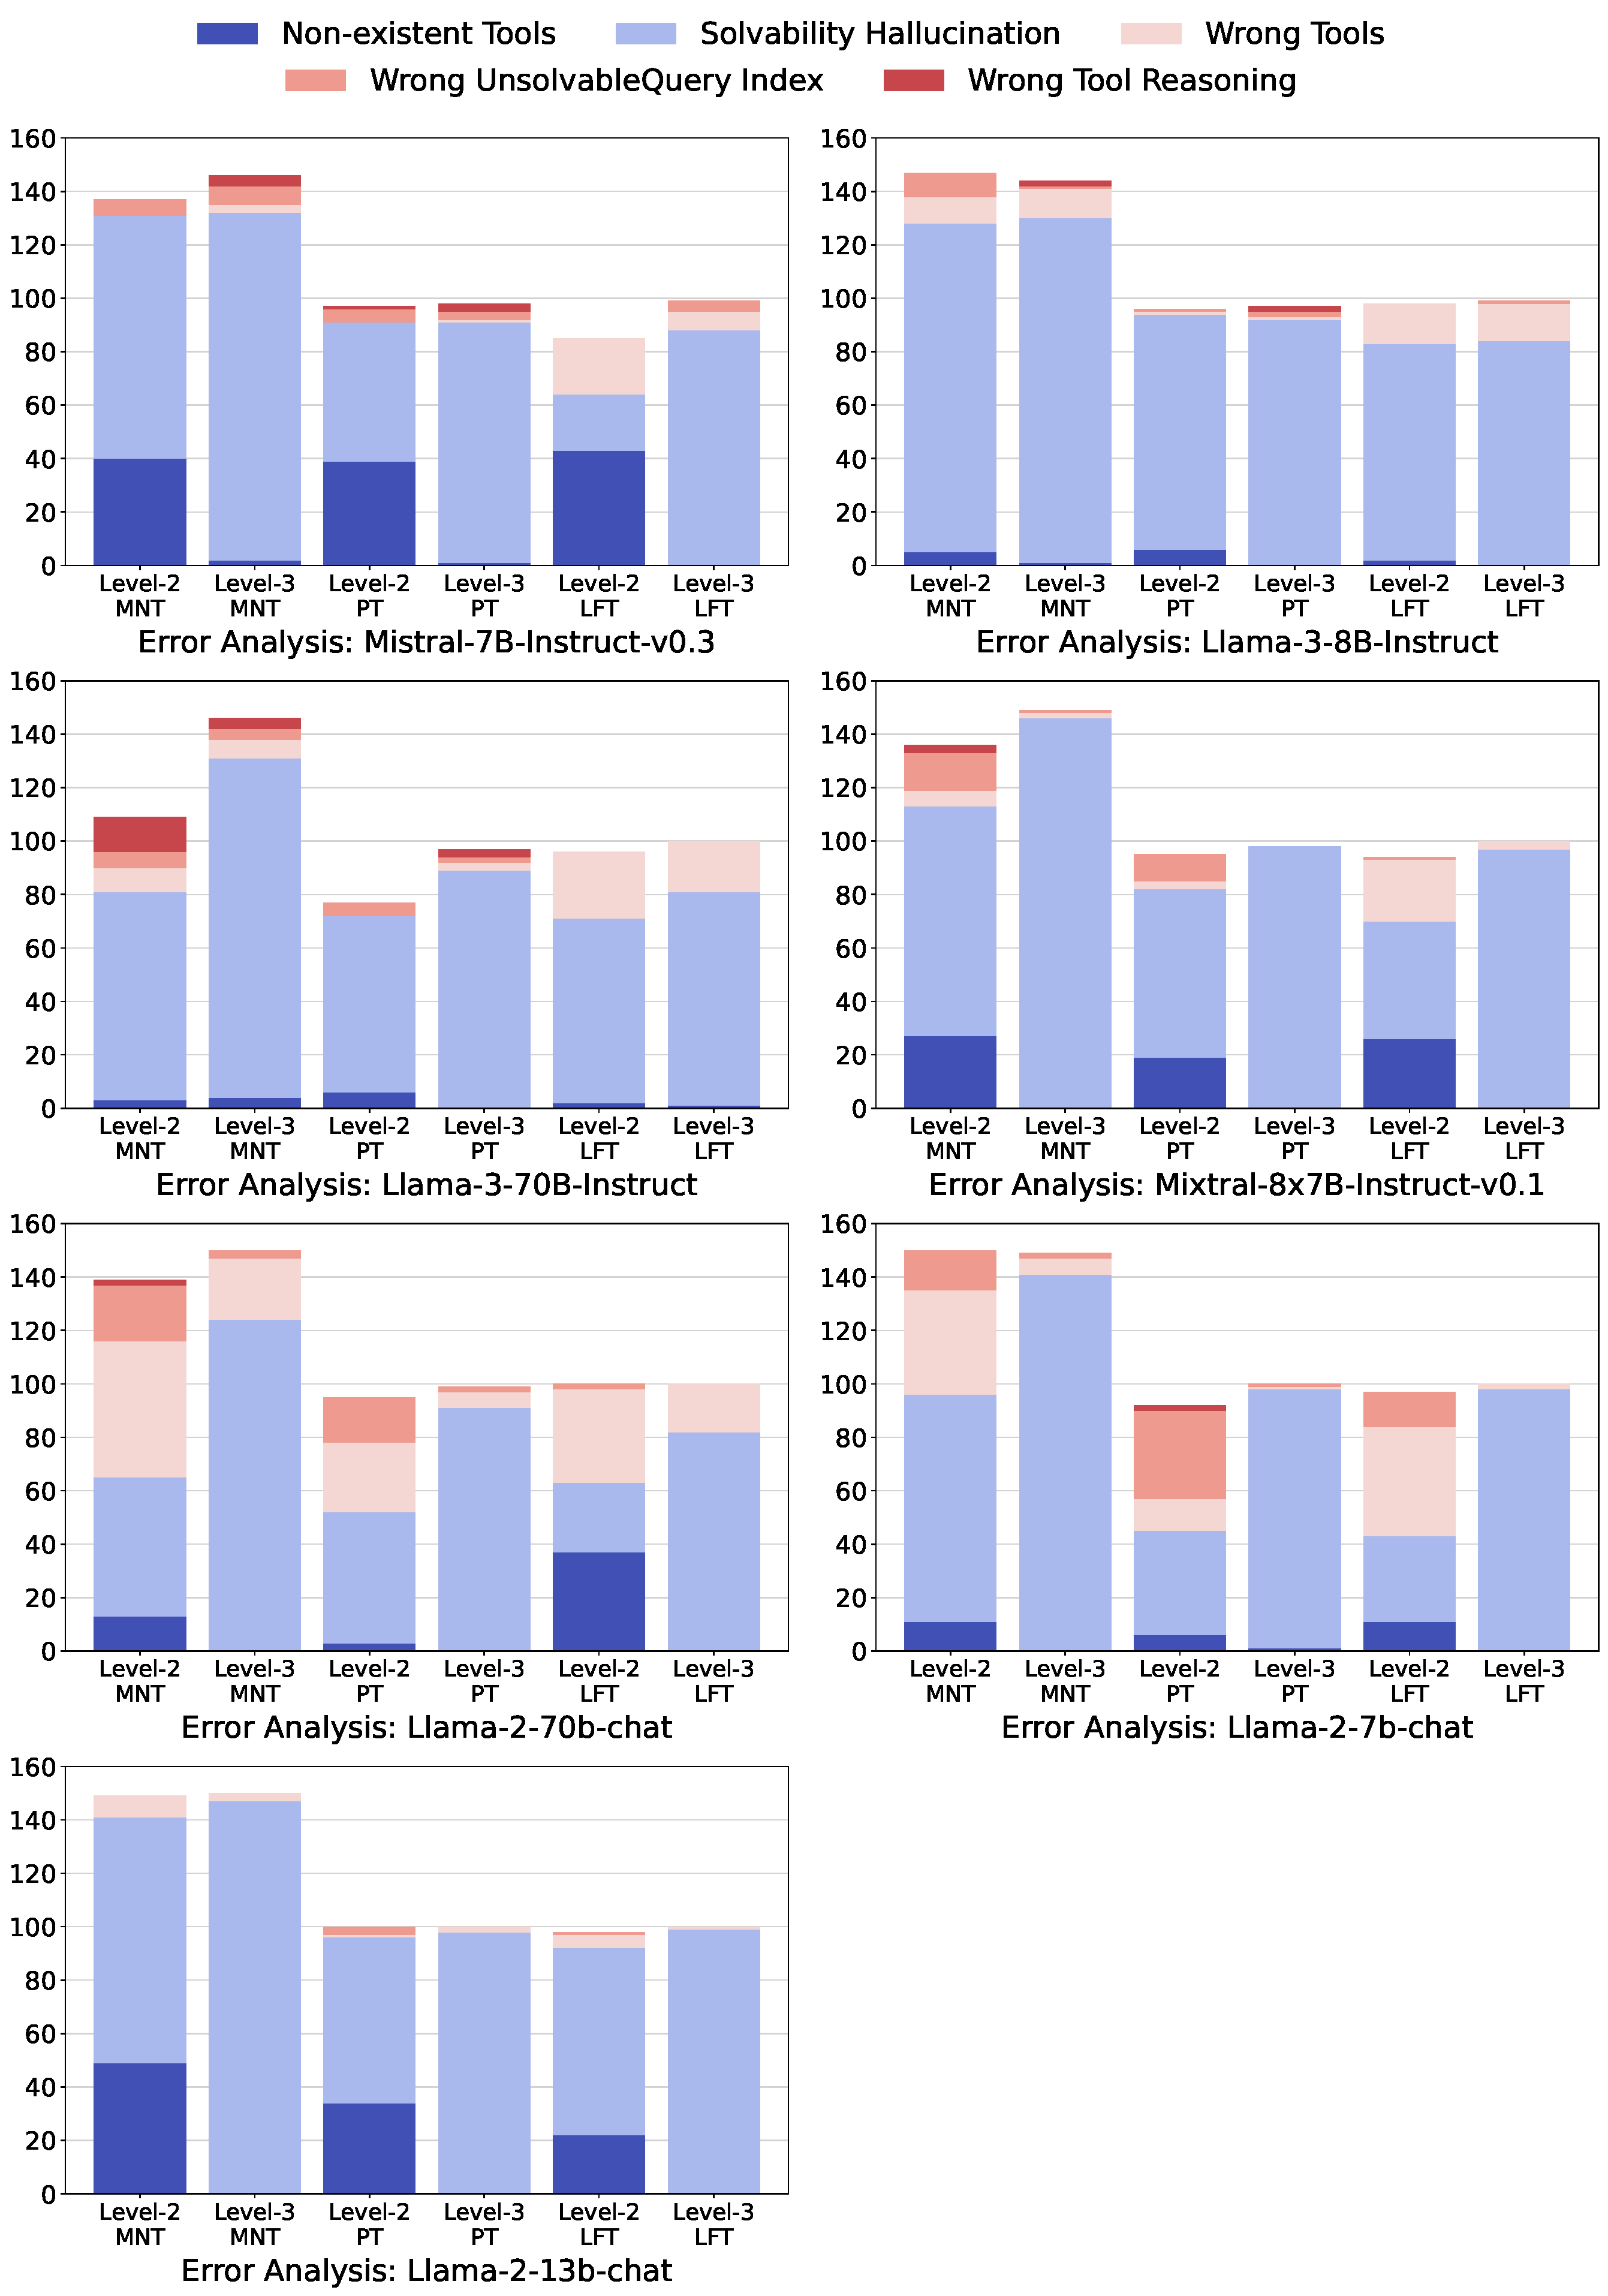
\includegraphics[width=0.98\textwidth]{figures/OS_models_all_error_analysis.pdf}
\caption{Error analysis for $7$ open-weight LLMs for Level-2 and Level-3 across three scenarios.
Scenarios: MNT (Missing Necessary Tools), PT (Potential Tools), and LFT (Limited Functionality Tools).}
\label{fig:error-analysis1}
\end{figure*}

\begin{figure*}[!tp]
\centering
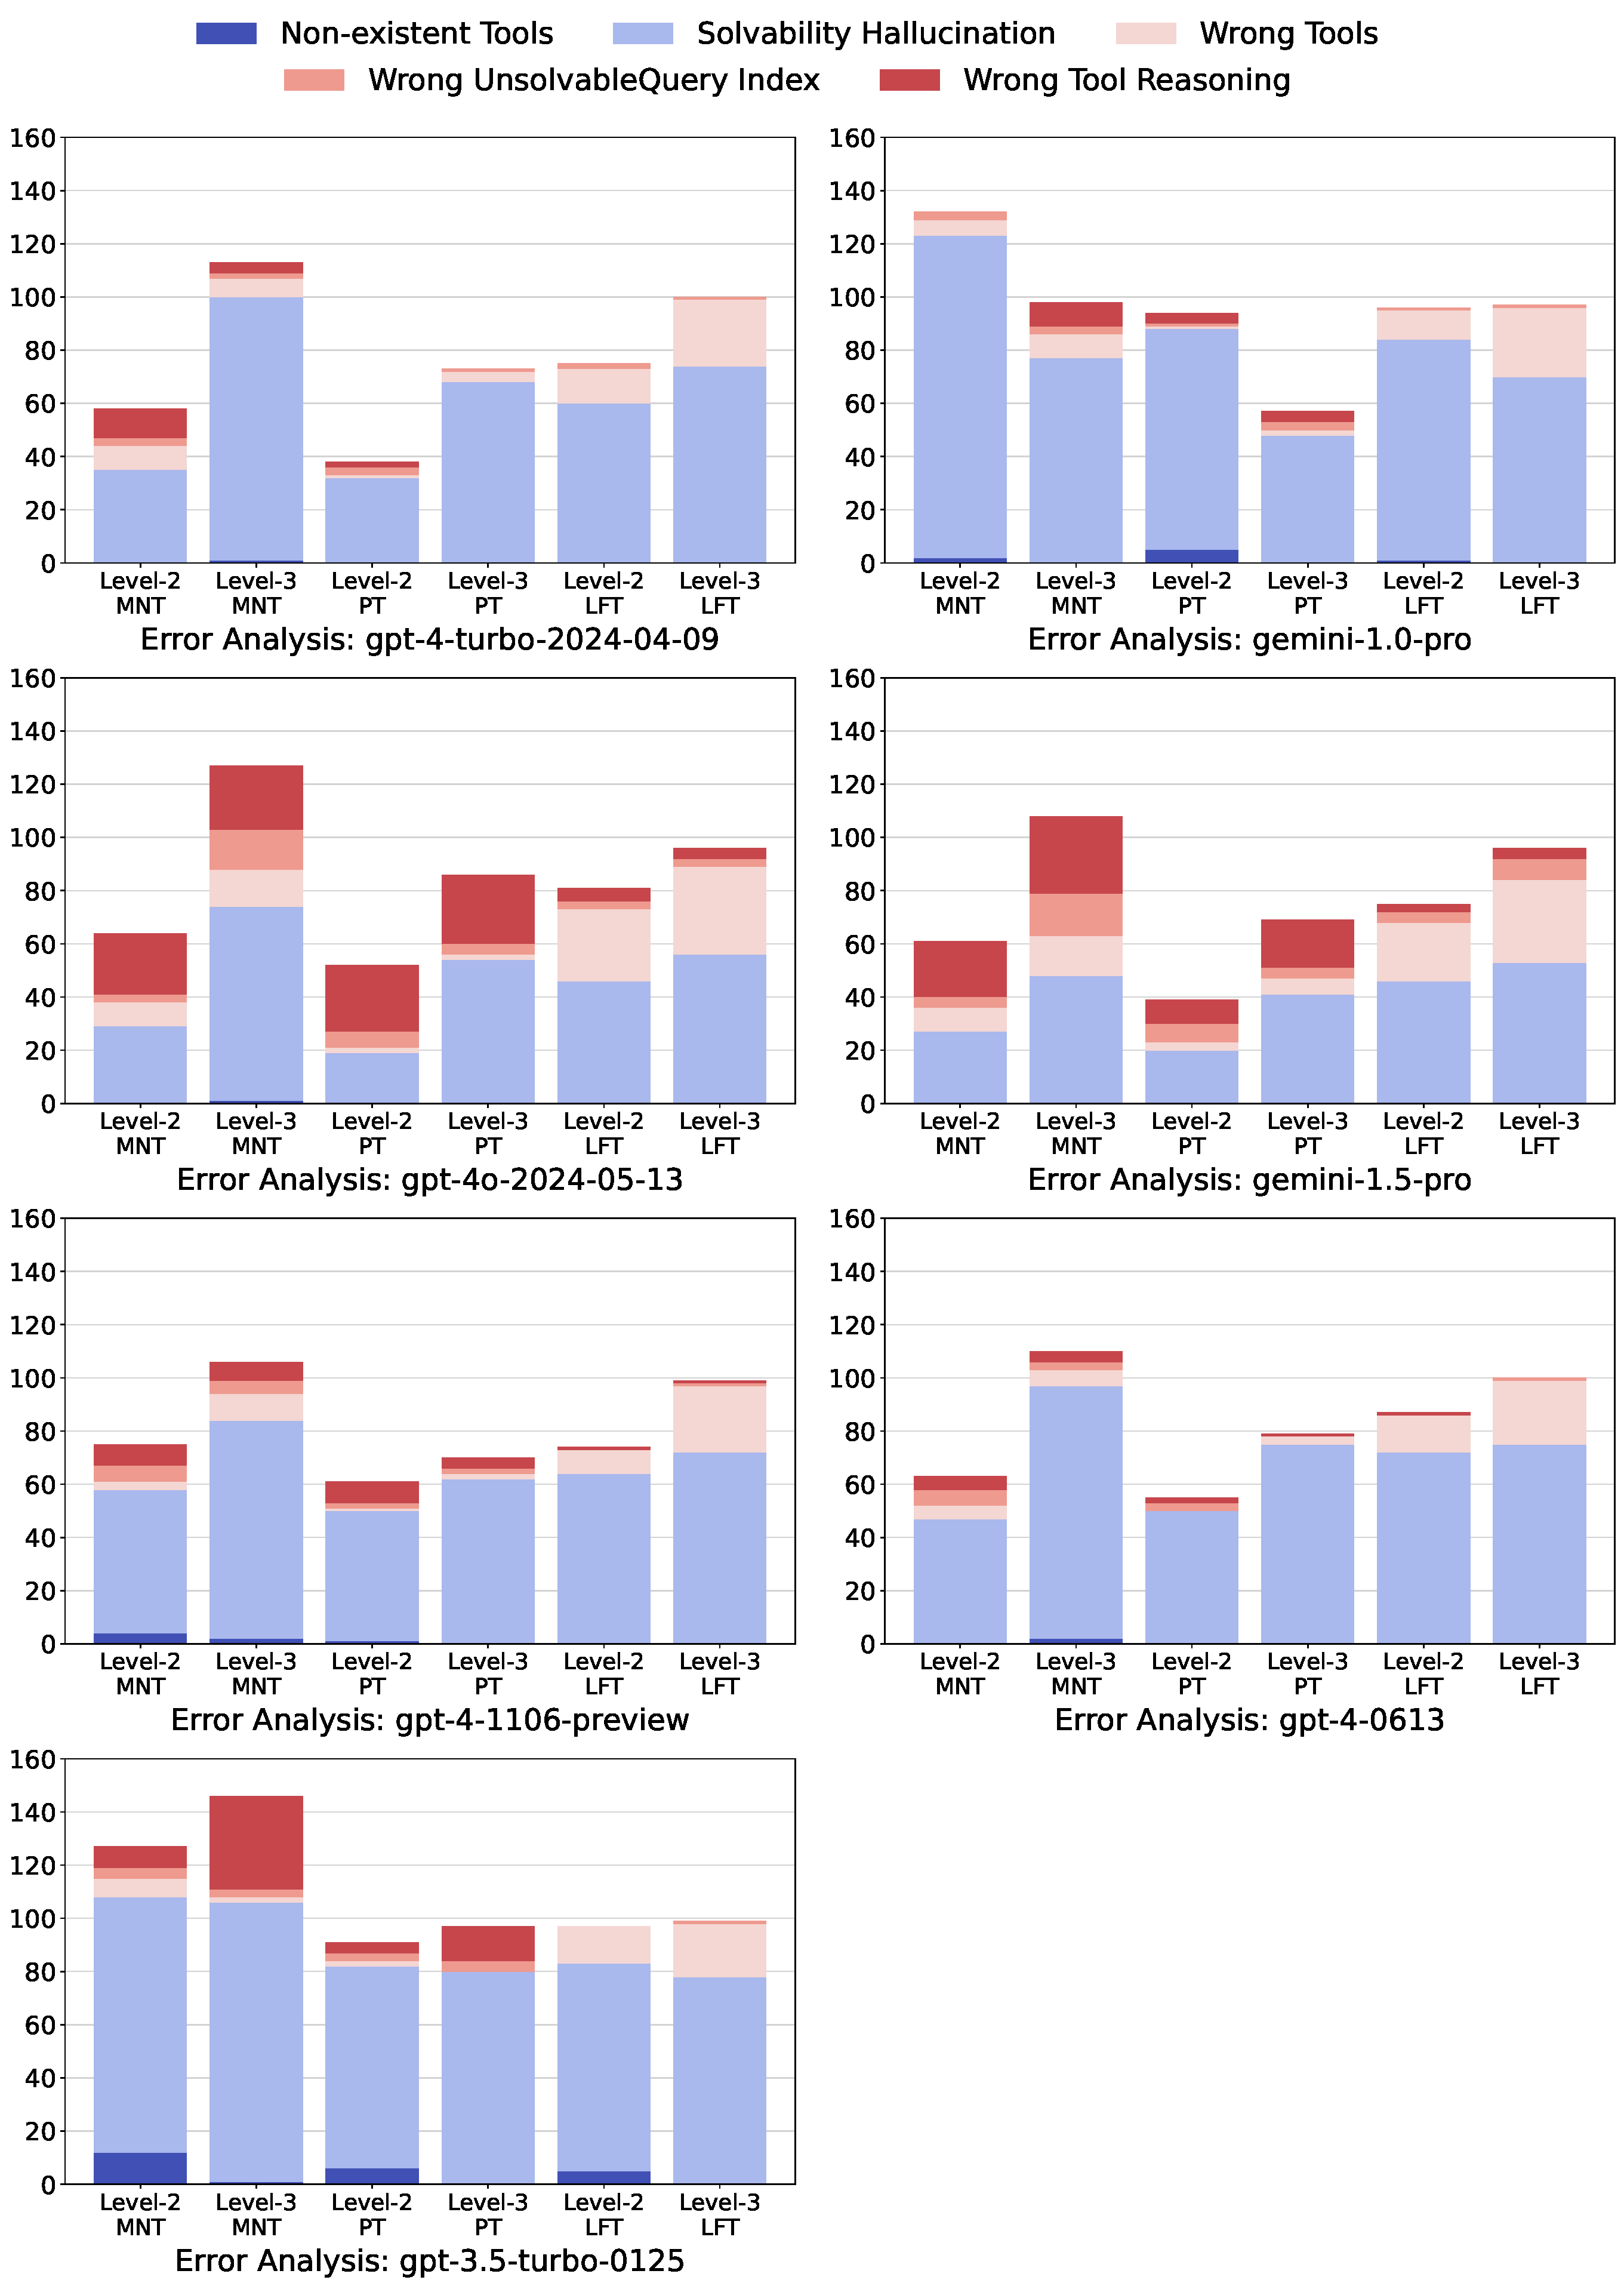
\includegraphics[width=0.98\textwidth]{figures/CS_models_all_error_analysis.pdf}
\caption{Error analysis for $7$ proprietary LLMs for Level-2 and Level-3 across three scenarios.
Scenarios: MNT (Missing Necessary Tools), PT (Potential Tools), and LFT (Limited Functionality Tools).}
\label{fig:error-analysis2}
\end{figure*}


\section{Case Study}

\subsection{Potential Tools Failure}
\label{append:ss:potential-tool-failure}

Considering textually fictionalized environments in prompts, LLMs erroneously assume that specific tools are available when explicitly informed that they are not. 
For example, in Linux environment, LLMs might try to use the unprovided tools such as ``rm'' and ``ufw''.

As illustrated in~\cref{tab:reprompt}, the latest GPT-4o model is susceptible to the hallucination of potential tools.
Furthermore, we provide several anonymous chats for GPT-4o: \url{https://chatgpt.com/share/83aa37e7-d87d-4fbd-9307-1f45cf29212d}, and GPT-4: \url{https://chatgpt.com/share/c11566af-4410-42a3-a84d-939a445e228a}.

A possible explanation for this phenomenon lies in the training data, which likely includes extensive information about operating systems and their associated tools. 
When the model is prompted to operate within the context of an operating system, it may inadvertently activate neural pathways associated with a broad range of system tools.
This activation in LLMs might lead to the erroneously outputting commands for restricted tools (e.g., ``ufw'') that are typically part of the operating system despite explicit instructions to use only a provided toolset. 
This behavior suggests a challenge in maintaining strict adherence to the given constraints while leveraging its comprehensive knowledge of operating system environments.

\subsection{Different Response Strategies}
\label{append:ss:strategy}

As observed in~\cref{ss:error-analysis},``Solvability Hallucinations'' are significantly more prevalent in L3 than in L2, regardless of whether the model is proprietary or open-weight. 
This is attributed to the additional missing-tool analysis in L3, which may lead the model to generate its content while disregarding certain inherent limitations associated with the task and tool.
Similarly, we endeavor to extend this conjecture to different models for further analysis.
In our experiments, we observe that even when a prompt explicitly requests that the model refrain from producing any output other than what is requested, some models may still exhibit unnecessarily conversational enthusiasm and generate replies with highly redundant content. 
This phenomenon is likely attributable to both the format of the training data and the response preferences. 
We present several examples from~\cref{tab:hot_response_lv1} to~\cref{tab:hot_response_lv3}.
Since we require the use of the tags <answer> and </answer> to delineate the answer part in the prompt, it is convenient for us to match answers to this class of "over-enthusiastic" models.
However, we discover that models with more redundant responses were less accurate than models that adhered to the construct of replying only to the answer part, as discussed in~\cref{append:pred_length}, and this phenomenon was independent of the model parameter size.
For example, we observe that Llama-2 responses exhibited a greater level of enthusiasm than Llama-3. 
For similar parameters, Llama-3 demonstrates a significant performance advantage over Llama-2; notably, the Llama-3-8B model even surpasses the Llama-2-70B in overall score.
This phenomenon suggests that in tool-augmented LLM, the setting of training data and the construction of response preference-aligned data have an equally non-negligible impact on task performance.


\subsection{Analysis of Continual Instructions}
\label{append:ss:reprompt}

We observed that LLMs sometimes fail to initially identify an unsolvable problem correctly but can be guided to the correct answer with additional human prompts. 
As illustrated in~\cref{tab:reprompt}, GPT-4 provides the correct answer after an additional round of prompt.
This indicates that LLMs have the capability to generate correct responses, provided they receive appropriate prompts.
However, as shown in~\cref{tab:reprompt}, GPT-4o still struggle with hallucinations.
Considering that additional prompts generally exist in multi-turn dialogue data, we hypothesize that the specific aspects of the training data and multi-turn dialogue training strategies may contribute to this issue.

\subsection{Consistency in Contextual Reasoning}
\label{append:ss:consistency}

As shown in~\cref{tab:consistency}, the results indicate that the Gemini-1.5-Pro exhibits greater consistency in self-contextual reasoning in unsolvable scenarios between Level-2 and Level-3, compared to the GPT-4o. 
Specifically, at Level-2, Gemini-1.5-Pro's responses show that the second task requirement is unsolvable and outputs an ``UnsolvableQuery''. 
In the same task at Level-3, Gemini-1.5-Pro's response continues to predict an ``UnsolvableQuery'' as the planned tool for subgoal 2. 
In contrast, while GPT-4o's response successfully predicts an ``UnsolvableQuery'' at Level-2, at Level-3, it bypassed the originally unsolvable subgoal and proceeded directly with subsequent task planning.
Therefore, it can be hypothesized that the Gemini-1.5-Pro possesses a better understanding of the implications of ``UnsolvableQuery'' and the actual solvability of tasks, and this understanding is not affected by changes in task demands or the context of the model's self-reasoning.
Conversely, when detailed task planning is conducted concurrently with the execution of tasks, GPT-4o is more likely to be influenced by the context content it reasons out, leading to deviations in subsequent task planning from the prescribed task requirements.

\newcolumntype{Y}[1]{%
  >{\small\everypar{\hangindent=1em}\arraybackslash}p{#1}%
}
\onecolumn
\begin{table}[!tp]
\small
\caption{Continual instructions analysis. In this case, GPT-4 successfully provides the correct answer when given further prompts, whereas the newer model, GPT-4o, fails to do so.}
\begin{tabular}{@{}Y{0.95\linewidth}@{}}
\toprule
\textbf{User Query} \\
\colorbox{blue!20}{<Level-1 Instruction>}\\
\\
<task>\\
Requirements for modifying system settings to enhance security in the Ubuntu Linux operating system environment:\\
1. Installation of firewalls;\\
2. Disable unneeded ports;\\
3. Enable access control;\\
4. Set up automatic updates.\\
</task>\\
\\
<provided\_tools>\\
1. PortManager: Manages ports.\\
2. AccessController: Manages access control.\\
3. AutoUpdater: Manages automatic system updates.\\
4. ReportGenerator: Generates a report with completed tasks.\\
5. Finish: Used to end the task.\\
6. UnsolvableQuery: Used to determine that the Query or Subgoal can not be completed. \\
</provided\_tools>\\
\midrule
% \midrule
\textbf{GPT-4's response}\\
\colorbox{green!20}{<answer>solvable</answer>}\\
\\
\textbf{GPT-4o's response}\\
\colorbox{red!20}{<answer>solvable</answer>}\\
\midrule
\midrule
\textbf{Reprompt}\\
How will you solve the first requirement: ``1. Installation of firewalls'' ? \\

\midrule
\textbf{GPT-4's response}\\
\colorbox{green!20}{<answer>unsolvable</answer>}\\
\\
\textbf{GPT-4o's response}\\
To solve the first requirement, ``Installation of firewalls'', in an \colorbox{red!20}{Ubuntu Linux operating system environment} using the tools provided, I will follow these steps:\\
Step-by-Step Solution:\\
\quad Check Current Firewall Status:\\

\quad \quad Before installing a firewall, I will ...\\
\quad Install the Firewall:\\

\quad \quad If no firewall is found or ...\\
\quad Detailed Execution Plan:\\
\quad \quad ...\\
\quad \quad Use the Finish tool to end the task after all requirements are met.
By following these steps, I will ensure that a firewall is installed, enabled, and properly configured to enhance the security of the Ubuntu system.\\
\bottomrule
\vspace{-2em}
\label{tab:reprompt}
\end{tabular}
\end{table}
\twocolumn
% \newcolumntype{Y}[1]{%
%   >{\small\everypar{\hangindent=1em}\arraybackslash}p{#1}%
% }
\onecolumn
\begin{table}[!tp]
\small
\caption{Responses of five different models in the PT scenario Level-1.}
\begin{tabular}{@{}Y{0.95\linewidth}@{}}
\toprule
\textbf{User Query} \\
\colorbox{blue!20}{<Level-1 Instruction>} \\
\\
<task>\\
Requirements for modifying system settings to enhance security in the Ubuntu Linux operating system environment:\\
1. Installation of firewalls;\\
2. Disable unneeded ports;\\
3. Enable access control;\\
4. Set up automatic updates.\\
</task>\\
\\
<provided\_tools>\\
1. PortManager: Manages ports.\\
2. AccessController: Manages access control.\\
3. AutoUpdater: Manages automatic system updates.\\
4. ReportGenerator: Generates a report with completed tasks.\\
5. Finish: Used to end the task.\\
6. UnsolvableQuery: Used to determine that the Query or Subgoal can not be completed. \\
</provided\_tools>\\
\midrule
\midrule
\textbf{GPT-4o's response}\\
<answer>solvable</answer>\\
\\
\textbf{Gemini-1.5-Pro's response}\\
<answer>solvable</answer>\\
\\
\textbf{Llama-3-70B's response}\\
<answer>solvable</answer>\\
\\
\textbf{Llama-2-70B's response}\\
<answer>solvable</answer>\\
The task requirements for modifying system settings to enhance security in the Ubuntu Linux operating system environment can be fulfilled with the tools provided.\\
1. Installation of firewalls: PortManager can be used to manage ports and install firewalls.\\
2. Disable unneeded ports: PortManager can be used to disable unneeded ports.\\
3. Enable access control: AccessController can be used to manage access control.\\
4. Set up automatic updates: AutoUpdater can be used to set up automatic system updates.\\
Therefore, all the task requirements can be completed with the tools provided, making the task solvable.\\
\bottomrule
\label{tab:hot_response_lv1}
\vspace{-2em}
\end{tabular}
\end{table}
\twocolumn

% \newcolumntype{X}[1]{%
%   >{\small\everypar{\hangindent=1em}\arraybackslash}p{#1}%
% }
\onecolumn
\begin{table}[!tp]
\small
\caption{Responses of five different models in the PT scenario Level-2.}
\begin{tabular}{@{}Y{0.95\linewidth}@{}}
\toprule
\textbf{User Query} \\
\colorbox{blue!20}{<Level-2 Instruction>}\\
\\
<task>\\
Requirements for modifying system settings to enhance security in the Ubuntu Linux operating system environment:\\
1. Installation of firewalls;\\
2. Disable unneeded ports;\\
3. Enable access control;\\
4. Set up automatic updates.\\
</task>\\
\\
<provided\_tools>\\
1. PortManager: Manages ports.\\
2. AccessController: Manages access control.\\
3. AutoUpdater: Manages automatic system updates.\\
4. ReportGenerator: Generates a report with completed tasks.\\
5. Finish: Used to end the task.\\
6. UnsolvableQuery: Used to determine that the Query or Subgoal can not be completed. \\
</provided\_tools>\\
\midrule
\midrule
\textbf{GPT-4o's response}\\
<answer>UnsolvableQuery$\backslash$nPortManager$\backslash$nAccessController$\backslash$nAutoUpdater$\backslash$nFinish</answer>\\
\\
\textbf{Gemini-1.5-Pro's response}\\
<answer>$\backslash$nUnsolvableQuery$\backslash$nPortManager$\backslash$nAccessController$\backslash$nAutoUpdater$\backslash$nReportGenerator$\backslash$nFinish$\backslash$n</answer>\\
\\
\textbf{Llama-3-70B's response}\\
<answer>PortManager$\backslash$nAccessController$\backslash$nAutoUpdater$\backslash$nFinish</answer>\\
Explanation:\\
1. Installation of firewalls: Although there is no specific tool for firewall installation, PortManager can be used to manage ports, which is related to firewall configuration. If a specific firewall installation tool is not available, UnsolvableQuery could be used, but in this case, PortManager can be used as a substitute.\\
2. Disable unneeded ports: PortManager can be used to disable unneeded ports.\\
3. Enable access control: AccessController can be used to enable access control.\\
4. Set up automatic updates: AutoUpdater can be used to set up automatic updates.\\
5. Finish: The Finish tool is used to end the task.\\
Note: ReportGenerator is not needed in this task, and UnsolvableQuery is not required since all steps can be completed with the available tools.\\
\\
\textbf{Llama-2-70B's response}\\
<answer>$\backslash$nPortManager$\backslash$nAccessController$\backslash$nAutoUpdater$\backslash$nFinish$\backslash$n</answer>\\
Explanation:\\
1. Installation of firewalls: PortManager\\
2. Disable unneeded ports: PortManager\\
3. Enable access control: AccessController\\
4. Set up automatic updates: AutoUpdater\\
5. Report generation (optional): ReportGenerator\\
6. Task completion: Finish\\
Note: The task does not require the use of the UnsolvableQuery tool, as all steps can be completed with the provided tools.\\
\bottomrule
\vspace{-2em}
\label{tab:hot_response_lv2}
\end{tabular}
\end{table}
\twocolumn

% \newcolumntype{Y}[1]{%
%   >{\small\everypar{\hangindent=1em}\arraybackslash}p{#1}%
% }
\onecolumn
\begin{table}[!tp]
\small
\caption{Responses of five different models in the PT scenario Level-3. Some lengthy
content is omitted with ``. . .'' for brevity.}
\begin{tabular}{@{}Y{\textwidth}@{}}
\toprule
\textbf{User Query} \\
\colorbox{blue!20}{<Level-3 Instruction>}\\
\\
<task>\\
Requirements for modifying system settings to enhance security in the Ubuntu Linux operating system environment:\\
1. Installation of firewalls;\\
2. Disable unneeded ports;\\
3. Enable access control;\\
4. Set up automatic updates.\\
</task>\\
\\
<provided\_tools>\\
1. PortManager: Manages ports.\\
2. AccessController: Manages access control.\\
3. AutoUpdater: Manages automatic system updates.\\
4. ReportGenerator: Generates a report with completed tasks.\\
5. Finish: Used to end the task.\\
6. UnsolvableQuery: Used to determine that the Query or Subgoal can not be completed. \\
</provided\_tools>\\
\midrule
\midrule
\textbf{GPT-4o's response}\\
<answer>$\backslash$nSubgoal 1: Install firewalls to enhance security. Planned tool: UnsolvableQuery$\backslash$nSubgoal 2: Disable unneeded ports to reduce potential attack vectors. Planned tool: PortManager$\backslash$nSubgoal 3: Enable access control to restrict unauthorized access. Planned tool: AccessController$\backslash$nSubgoal 4: Set up automatic updates to ensure the system is up-to-date with security patches. Planned tool: AutoUpdater$\backslash$nSubgoal 5: [Task requires number of tools within 4] Planned tool: Finish$\backslash$n</answer>\\
\\
\textbf{Gemini-1.5-Pro's response}\\
<answer>$\backslash$nSubgoal 1: [Install firewalls to enhance security, requires a tool specifically designed for firewall management] Planned tool: UnsolvableQuery$\backslash$nSubgoal 2: [Disable unnecessary ports to enhance security] Planned tool: PortManager$\backslash$nSubgoal 3: [Enable access control to enhance security] Planned tool: AccessController $\backslash$nSubgoal 4: [Set up automatic updates to enhance security] Planned tool: AutoUpdater$\backslash$nSubgoal 5: [Generate a report of the completed tasks] Planned tool: ReportGenerator$\backslash$nSubgoal 6: [All tasks are completed] Planned tool: Finish $\backslash$n</answer>\\
\\
\textbf{Llama-3-70B's response}\\
<answer>$\backslash$nSubgoal 1: Install firewall to enhance system security Planned tool: PortManager$\backslash$nSubgoal 2: Disable unneeded ports to prevent unauthorized access Planned tool: PortManager$\backslash$nSubgoal 3: Configure access control to restrict access to system resources Planned tool: AccessController$\backslash$nSubgoal 4: Set up automatic updates to ensure system is up-to-date with security patches Planned tool: AutoUpdater$\backslash$nSubgoal 5: Generate a report to document completed tasks Planned tool: ReportGenerator$\backslash$nSubgoal 6: Task completion Planned tool: Finish$\backslash$n</answer>\\
In this task plan, each subgoal is logically related to the overall task of modifying system settings to enhance security in the Ubuntu Linux operating system environment. The tools used are only from the provided list, and each subgoal advances the overall task progress.\\
Subgoal 1 and 2 are related to securing the system by installing a firewall and disabling unneeded ports, which are both achieved using the PortManager tool.\\
Subgoal 3 is related to configuring access control, which is achieved using the AccessController tool.\\
Subgoal 4 is related to setting up automatic updates, which is achieved using the AutoUpdater tool.\\
Subgoal 5 is related to generating a report to document the completed tasks, which is achieved using the ReportGenerator tool.\\
Subgoal 6 marks the completion of the task, which is achieved using the Finish tool.\\
Note that the UnsolvableQuery tool is not used in this task plan, as the task can be completed using the provided tools.\\
\\
\textbf{Llama-2-70B's response}\\
<answer>$\backslash$nSubgoal 1: Install firewalls Planned tool: PortManager$\backslash$nSubgoal 2: Disable unnecessary ports Planned tool: PortManager$\backslash$nSubgoal 3: Enable access control Planned tool: AccessController$\backslash$nSubgoal 4: Set up automatic updates Planned tool: AutoUpdater$\backslash$nSubgoal 5: Generate a report with completed tasks Planned tool: ReportGenerator$\backslash$nSubgoal 6: End the task Planned tool: Finish$\backslash$n</answer>\\
Explanation:\\
1. Subgoal 1: Install firewalls\\
\quad \quad * Description: Installing firewalls is essential for enhancing security in the Ubuntu Linux operating system environment.\\
\quad \quad * Tool: PortManager\\
2. Subgoal 2: Disable unnecessary ports\\
\quad \quad * Description: Disabling unnecessary ports can help prevent potential security breaches.\\
\quad \quad * Tool: PortManager\\
...\\
Note:\\
* The tools provided in the <provided\_tools> section are the only tools that can be used in the task.\\
* The subgoals are logically related to each other, and completing each subgoal advances the overall task progress.\\
* The number of tools used in the task is limited to 6, which is the number of tools provided in the <provided\_tools> section. If more tools were needed, the task would terminate with UnsolvableQuery.\\
\bottomrule
\label{tab:hot_response_lv3}
\vspace{-2em}
\end{tabular}
\end{table}
\twocolumn



\newcolumntype{Y}[1]{%
  >{\small\everypar{\hangindent=1em}\arraybackslash}p{#1}%
}
\onecolumn
\begin{table}[!tp]
\small
\caption{Gemini series models show better consistency in contextual reasoning between Level-2 and Level-3.}
\begin{tabular}{@{}Y{\textwidth}@{}}
\toprule
\textbf{User Query} \\
\colorbox{blue!20}{<Level-2 and Level-3 Instruction>}\\
\\
<task>\\
Modify the kernel version of the computer in a Linux operating system environment. Do the following.\\
1. Download the kernel update package.\\
2. Update the kernel version.\\
3. Restart the computer.\\
</task>\\
\\
<provided\_tools>\\
1. KernelDownloader: Download kernel update packages on Linux systems.\\
2. Restart: Restarts the computer in a Linux system.\\
3. Finish: Used to end the task.\\
4. UnsolvableQuery: Used to determine that the Query or Subgoal can not be completed
</provided\_tools>\\
\midrule
\midrule
\textbf{GPT-4o's response in Level-2}\\
<answer>KernelDownloader$\backslash$n\colorbox{red!20}{UnsolvableQuery}$\backslash$nRestart$\backslash$nFinish</answer>\\
\\
\textbf{GPT-4o's response in Level-3}\\
<answer>Subgoal 1: [Download the kernel update package to prepare for the kernel update] Planned tool: KernelDownloader$\backslash$n\colorbox{red!20}{Subgoal 2: [Restart the computer to apply the new kernel version] Planned tool: Restart}$\backslash$nSubgoal 3: [End the task after the computer restarts] Planned tool: Finish</answer>\\
\\
\midrule
\textbf{Gemini-1.5-Pro's response in Level-2}\\
<answer>KernelDownloader$\backslash$n\colorbox{green!20}{UnsolvableQuery}$\backslash$nRestart$\backslash$nFinish</answer>\\
\textbf{Gemini-1.5-Pro's response in Level-3}\\
<answer>Subgoal 1: Download the kernel update package. Planned tool: KernelDownloader$\backslash$n\colorbox{green!20}{Subgoal 2: Update the kernel}\\ \colorbox{green!20}{version. Planned tool: UnsolvableQuery}$\backslash$nSubgoal 3: Restart the computer. Planned tool: Restart$\backslash$nSubgoal 4: End the task. Planned tool: Finish</answer>\\
\bottomrule
\label{tab:consistency}
\vspace{-2em}
\end{tabular}
\end{table}
\twocolumn



\begin{figure*}[!htb]
\small
\begin{tcolorbox}[
    colback=white, 
    colframe=blue1, 
    boxrule=0.5mm,
    arc=0mm,
    outer arc=0mm,
    title=Missing Necessary Tools: Single-step - Generation Prompt]
Task Description:\\
You need to go ahead and generate samples of tool usage with as much diversity as possible, based on the current dimension, the requirements requirements of the task, and the sample references provided.\\

Current dimension:\\
Single-step tool using: the case where the output tool is directly requested in single-step reasoning\\

Task Requirement:\\
- Generate new samples with as much diversity as possible in terms of user query and available tools.\\
- Use "// Raw Input //" and "// Raw Output //" to label the inputs and outputs of the samples.\\
- The sample needs to consider a real-life scenario as much as possible. Multiple tools need to be provided in the raw input, and in the current dimension, the raw output uses only one tool to fulfill the user's query in the planning phase, which corresponds to Single-step tool using.\\

At build time, you need to:\\
First give a copy of the overall task, which usually has only a single requirement. In the list of available tools, make sure to provide tools that can fulfill this requirement, while adding a small number of tools that do not directly contribute to the task to ensure task complexity and tool diversity. Finally, complete the corresponding task planning process in the output based on these requirements, keeping in mind that only one tool was used to accomplish the task.\\

Sample Reference:\\
==== Reference Sample Start ====\\
// Raw Input //\\
\colorbox{blue1!50}{\texttt{[sample\_input]}}\\

// Raw output //\\
\colorbox{blue1!50}{\texttt{[sample\_outputl]}}\\
==== Reference Sample End ====\\

Now, please combine the reference sample and the corresponding build steps, try to select tasks from different domains and scenarios, and use different types of tools to make the new sample different from the reference sample in terms of task content and context. We start generating new single samples corresponding to the dimensions.\\
Single-step tool using dimension generation sample (one):\\
==== Sample start ====
\end{tcolorbox}
\caption{Generation prompt for missing necessary tools scenario, single-step subtask.}
\label{fig:single-step-prompt}
\end{figure*}
\begin{figure*}[!htb]
\small
\begin{tcolorbox}[
    colback=white, 
    colframe=blue1, 
    boxrule=0.5mm,
    arc=0mm,
    outer arc=0mm,
    title=Missing Necessary Tools: Multi-step w/o Repetition - Generation Prompt
]
Task Description:\\
You need to go ahead and generate samples of tool usage with as much diversity as possible, based on the current dimension, the requirements requirements of the task, and the sample references provided.\\

Current dimension:\\
Multi-step tool using w/o Repetition: no repetitive tool calls, each call in the process is a different tool\\

Task Requirement:\\
- Generate new samples taking into account as much as possible the diversity of user query and available tools.\\
- First, ensure that the task description is a goal that requires the use of multiple tools to accomplish, and provide the corresponding tools in the list of available tools, using numerical numbers. Then make sure that all tools are invoked only once during the planning phase.\\
- Use "// Raw Input //" and "// Raw Output //" to label the inputs and outputs of the samples.\\
- The samples need to consider a realistic scenario as much as possible, multiple tools need to be provided in the raw input, in the current dimension, the raw output uses multiple tools to fulfill the user's query in the planning phase, which corresponds to Multi-step tool using. and in the invocation process, different tools are used in each step, which corresponds to w/o Repetition\\

At build time, you need to:\\
First give a list of overall tasks and then express specific task requirements separately. In the list of available tools, make sure that you provide tools that can fulfill these requirements, and include a small number of tools that do not directly contribute to the task to ensure task complexity and tool diversity. Finally, complete the corresponding task planning process in the output based on these requirements, keeping in mind that each step corresponds to a different tool.\\

Sample Reference:\\
==== Reference Sample Start ====\\
// Raw Input //\\
\colorbox{blue1!50}{\texttt{[sample\_input]}}\\

// Raw output //\\
\colorbox{blue1!50}{\texttt{[sample\_outputl]}}\\
==== Reference Sample End ====\\

Now, please combine the reference sample and the corresponding build steps, try to select tasks from different domains and scenarios, and use different types of tools to make the new sample different from the reference sample in terms of task content and context. We start generating new single samples corresponding to the dimensions.\\
Multi-step tool using w/o Repetition dimension generation sample (one):\\
==== Sample Start ====
\end{tcolorbox}
\caption{Generation prompt for missing necessary tools scenario, multi-step w/o repetition subtask.}
\label{fig:multi-step-worep-prompt}
\end{figure*}
\begin{figure*}[!htb]
\small
\begin{tcolorbox}[
    colback=white, 
    colframe=blue1, 
    boxrule=0.5mm,
    arc=0mm,
    outer arc=0mm,
    title=Missing Necessary Tools: Multi-step w/ Repetition - Generation Prompt
]
Task Description:\\
You need to go ahead and generate samples of tool usage with as much diversity as possible, based on the current dimension, the requirements requirements of the task, and the sample references provided.\\

Current dimension:\\
Multi-step tool using w Repetition: the task needs to be completed using multiple steps and a tool has been called twice in the planning phase.\\

Task Requirement:\\
- Generate new samples taking into account as much as possible the diversity of user query and available tools.
- First, ensure that the task description is a goal that requires the use of multiple tools to accomplish, and provide the corresponding tools in the list of available tools using numerical numbers. Then make sure that a tool is called twice during the planning phase.
- Use "// Raw Input //" and "// Raw output //" to label the inputs and outputs of the samples.
- The samples need to consider a realistic scenario as much as possible, and multiple tools need to be provided in the raw inputs. In the current dimension, the raw outputs use multiple tools to fulfill the user's query in the planning phase, which corresponds to Multi-step tool using. and one tool is called twice in the planning phase, which corresponds to w Repetition\\

At build time, you need to:\\
First give a list of overall tasks and then express specific task requirements separately. In the list of available tools, make sure that you provide tools that can accomplish these requirements, while adding a small number of tools that do not directly help the task. Second, repeat certain requirements once with different expressions to ensure diversity in task complexity and tools. Finally, complete the corresponding task planning process in the output based on these requirements.\\

Sample Reference:\\
==== Reference Sample Start ====\\
// Raw Input //\\
\colorbox{blue1!50}{\texttt{[sample\_input]}}\\

// Raw output //\\
\colorbox{blue1!50}{\texttt{[sample\_outputl]}}\\
==== Reference Sample End ====\\

Now, please combine the reference sample and the corresponding build steps, try to select tasks from different domains and scenarios, and use different types of tools to make the new sample different from the reference sample in terms of task content and context. We start generating new single samples corresponding to the dimensions.\\
Multi-step tool using w Repetition dimension generation sample (one):\\
==== Sample Start ====
\end{tcolorbox}
\caption{Generation prompt for missing necessary tools scenario, multi-step w/ repetition subtask.}
\label{fig:multi-step-wrep-prompt}
\end{figure*}
\begin{figure*}[!htb]
\small
\begin{tcolorbox}[
    colback=white, 
    colframe=blue2,
    boxrule=0.5mm,
    arc=0mm,
    outer arc=0mm,
    title=Potential Tools: Operating System - Generation Prompt
]
Task Description:\\
You need to go ahead and generate samples of tool usage with as much diversity as possible, based on the current dimension, the requirements requirements of the task, and the sample references provided.\\

Current dimension:\\
Application Environment Dimension - Special Environment Constraints: Operating System (OS)\\

Task Requirement:\\
- Generate new samples taking into account as much as possible the diversity of user query and available tools.
- Use "// Raw Input //" and "// Raw output //" to label the inputs and outputs of the samples.
- The samples need to consider a realistic scenario as much as possible. Multiple tools need to be available in the list of available tools in the raw input. Please note that in the current dimension, the raw output takes place and occurs in the OS environment in the planning phase, and requires the setting of user query related to the OS level, e.g., kernel updates, user settings, software installation, file or folder handling, boot settings, permissions management for files and directories, etc.\\

At build time, you need to:\\
Start by giving an overall task, then express specific task requirements separately, and make sure that they are as relevant to the os environment as possible. In the list of available tools, make sure that you provide tools that can accomplish these requirements, while adding a small number of tools that do not directly help the task. Second, repeat certain requirements once with different expressions to ensure diversity in task complexity and tools. Finally, complete the corresponding task planning process in the output based on these requirements.\\

Sample Reference:\\
==== Reference Sample Start ====\\
// Raw Input //\\
\colorbox{blue2!50}{\texttt{[sample\_input]}}\\

// Raw output //\\
\colorbox{blue2!50}{\texttt{[sample\_outputl]}}\\
==== Reference Sample End ====\\

Now, please combine the reference sample and the corresponding build steps, try to select tasks from different domains and scenarios, and use different types of tools to make the new sample different from the reference sample in terms of task content and context. We start generating new single samples corresponding to the dimensions.\\
Special Environment Constraints: Operating System (OS) generation sample (one):\\
==== Sample Start ====
\end{tcolorbox}
\caption{Generation prompt for potential tools scenario, OS subtask.}
\label{fig:os-prompt}
\end{figure*}
\begin{figure*}[!htb]
\small
\begin{tcolorbox}[
    colback=white, 
    colframe=blue2,
    boxrule=0.5mm,
    arc=0mm,
    outer arc=0mm,
    title=Potential Tools: Web - Generation Prompt
]
Task Description:\\
You need to go ahead and generate samples of tool usage with as much diversity as possible, based on the current dimension, the requirements requirements of the task, and the sample references provided.\\

Current dimension:\\
Application Environment Dimension - Special Environment Constraints: Web\\

Task Requirement:\\
- Generate new samples taking into account as much as possible the diversity of user query and available tools.
- Use "// Raw Input //" and "// Raw output //" to label the inputs and outputs of the samples.
- The samples need to consider as much as possible a scenario that could happen in reality, and multiple tools need to be available in the raw input. In the current dimension, the task description is in a web-related environment, including but not limited to: shopping price comparison, web content retrieval, web data collection, website usability evaluation, website security evaluation, website optimization, etc.\\

At build time, you need to:\\
Give an overall task first, then express the specific task requirements separately, and make sure that they are as relevant to the web environment as possible. In the list of available tools, make sure that you provide tools that can accomplish these requirements, while including a small number of tools that do not directly help the task. Next, repeat certain requirements once with different expressions to ensure diversity in task complexity and tools. Finally, complete the corresponding task planning process in the output based on these requirements.\\

Sample Reference:\\
==== Reference Sample Start ====\\
// Raw Input //\\
\colorbox{blue2!50}{\texttt{[sample\_input]}}\\

// Raw output //\\
\colorbox{blue2!50}{\texttt{[sample\_outputl]}}\\
==== Reference Sample End ====\\

Now, please combine the reference sample and the corresponding build steps, try to select tasks from different domains and scenarios, and use different types of tools to make the new sample different from the reference sample in terms of task content and context. We start generating new single samples corresponding to the dimensions.\\
Special Environment Constraints: Web generation sample (one):\\
==== Sample Start ====
\end{tcolorbox}
\caption{Generation prompt for potential tools scenario, Web subtask,}
\label{fig:web-prompt}
\end{figure*}
\begin{figure*}[!htb]
\small
\begin{tcolorbox}[
    colback=white, 
    colframe=blue3, 
    boxrule=0.5mm,
    arc=0mm,
    outer arc=0mm,
    title=Limited Functionality Tools: Iterative - Generation Prompt
]
Task Description:\\
You need to go ahead and generate samples of tool usage with as much diversity as possible, based on the current dimension, the requirements requirements of the task, and the sample references provided.\\

Current dimension:\\
Iterative Dimension - The task requires repeated invocations of the same tool, with multiple iterations to get the final result\\

Task Requirement:\\
- Generate new samples taking into account as much as possible the diversity of user query and available tools.
- First ensure that the task description is a goal that requires the use of multiple tools to accomplish, and provide the corresponding tools in the list of available tools using numerical numbers. Then make sure that one tool is called more than twice in a row during the planning phase, and that this row of calls is reflected in the task planning.\\
- Use "// Raw Input //" and "// Raw output //" to label the inputs and outputs of the samples.\\
- The samples need to consider a realistic possible scenario as much as possible. Multiple tools need to be available in the list of available tools in the raw input. Note that in the current dimension, the raw output has multiple iterative calls to the same tool in the planning phase, with at least two or more steps in between, corresponding to the iterative call dimension.\\

At build time, you need to:\\
First give a list of overall tasks and then express specific task requirements separately. In the list of available tools, make sure to provide tools that can fulfill these requirements, while including a small number of tools that do not directly help the task to ensure task complexity and tool diversity. Second, by placing certain limitations on the tool capabilities that result in multiple invocations to accomplish a given requirement, and making these limitations and requirements explicit in the task description and the list of provided tools. Finally, the corresponding task planning process is completed in the output based on these requirements.\\

Sample Reference:\\
==== Reference Sample Start ====\\
// Raw Input //\\
\colorbox{blue3!50}{\texttt{[sample\_input]}}\\

// Raw output //\\
\colorbox{blue3!50}{\texttt{[sample\_outputl]}}\\
==== Reference Sample End ====\\

Now, please combine the reference sample and the corresponding build steps, try to select tasks from different domains and scenarios, and use different types of tools to make the new sample different from the reference sample in terms of task content and context. We start generating new single samples corresponding to the dimensions.\\
Iterative dimension generation sample (one):\\
==== Sample Start ====
\end{tcolorbox}
\caption{Generation prompt for limited functionality tools scenario, iterative subtask.}
\label{fig:iter-prompt}
\end{figure*}
\begin{figure*}[!htb]
\small
\begin{tcolorbox}[
    colback=white, 
    colframe=blue3,
    boxrule=0.5mm,
    arc=0mm,
    outer arc=0mm,
    title=Limited Functionality Tools: Optimal Tool Selection - Generation Prompt
]
Task Description:\\
You need to go ahead and generate samples of tool usage with as much diversity as possible, based on the current dimension, the requirements requirements of the task, and the sample references provided.\\

Current dimension:\\
Multiple Appropriate Tools Dimension - Optimal Tool Selection\\

Task Requirement:\\
- Generate new samples taking into account as much as possible the diversity of user query and available tools.
- First, make sure that the task description is a goal that requires the use of multiple tools to accomplish, and provide the corresponding tools in the list of available tools using numerical numbers.\\
- Use "// Raw Input //" and "// Raw output //" to label the inputs and outputs of the samples.\\
- The samples need to consider a realistic scenario as much as possible. Multiple tools need to be available in the list of available tools in the raw input. Note that there will be multiple suitable tools that all take on the same or very similar functions in the current dimension, e.g., for a language detection task, tool A may have a higher recognition rate for some minor languages, while tool B is more accurate on common languages. One needs to be weighed against the specific needs of the task (whether comprehensiveness is more important or accuracy for a particular language is more important); for a text sentiment analysis task, tool C can provide simple keyword-based sentiment analysis, while tool D is capable of deeper sentiment understanding and contextual analysis. In this case, if the user needs a quick and shallow analysis, tool C may be preferred; if deeper sentiment understanding is needed, tool D may be preferred. One needs to choose the right tool based on the specific situation, e.g., the complexity of the text and the detailed needs of the user; and so on.\\

At build time, you need to:\\
First give a list of overall tasks and then express specific task requirements separately. In the list of available tools, make sure to provide tools that can fulfill these requirements, while adding a small number of tools that do not directly help the task to ensure the complexity of the task and the diversity of tools. At the same time, in the current dimension, you need to build multiple tools with the same functionality but different focuses, and emphasize a particular focus in the task description to achieve the effect of selecting the most effective tool. Finally, according to these requirements, complete the corresponding task planning process in the output, keeping in mind that each step corresponds to a different tool.\\

Sample Reference:\\
==== Reference Sample Start ====\\
// Raw Input //\\
\colorbox{blue3!50}{\texttt{[sample\_input]}}\\

// Raw output //\\
\colorbox{blue3!50}{\texttt{[sample\_outputl]}}\\
==== Reference Sample End ====\\
Now, please combine the reference sample and the corresponding build steps, try to select tasks from different domains and scenarios, and use different types of tools to make the new sample different from the reference sample in terms of task content and context. We start generating new single samples corresponding to the dimensions.\\
Multiple Appropriate Tools Dimension - Optimal Tool Selection generation sample (one):\\
==== Sample Start ====
\end{tcolorbox}
\caption{Generation prompt for limited functionality tools scenario, optimal tool selection subtask.}
\label{fig:best-prompt}
\end{figure*}
\begin{figure*}[!htb]
\small
\begin{tcolorbox}[
    colback=white, 
    colframe=pink1,
    boxrule=0.5mm,
    arc=0mm,
    outer arc=0mm,
    title=Evaluation Prompt for Level-1 Solvability Detection
]
Determines whether the current task can be solved with the tools provided in <provided\_tools>, based on the task description in <task>. Note that you need to carefully review the requirements, limitations of the <task>, and capability descriptions of the tools in <provided\_tools>, and that you can't use tools that aren't provided in <provided\_tools>. \\
You need to wrap your answer in <answer> and </answer>. \\
If the task can be solved, output '<answer>solvable</answer>'. If the task is not solvable, output '<answer>unsolvable</answer>'. Other than that, do not output anything extra.\\
\\
<task>\\
\colorbox{pink1!50}{\texttt{[task\_description]}}\\
</task>\\
\\
<provided\_tools>\\
\colorbox{pink1!50}{\texttt{[provided\_tool\_list]}}\\
</provided\_tools>\\
\\
\end{tcolorbox}
\caption{Evaluation Prompt for Level-1 Solvability Detection}
\label{fig:level-1_prompt}
\end{figure*}
\begin{figure*}[!htb]
\small
\begin{tcolorbox}[
    colback=white, 
    colframe=pink2,
    boxrule=0.5mm,
    arc=0mm,
    outer arc=0mm,
    title=Evaluation Prompt for Level-2 Solution Planning
]
Plan your tool usage based on the task description in <task> and the available tools provided in <provided\_tools>. List the names of the tools you need to use to complete the task in order, wrapping them in <answer> and </answer> and separating each tool with a line break “$\backslash$n”, e.g.: \\
<answer>Tool1$\backslash$nTool2$\backslash$n... $\backslash$nTooln</answer>\\
\\
If a step of the task does not have a tool that can be solved in the list of tools provided by <provided\_tools>, use the UnsolvableQuery tool at the corresponding step, and then continue the planning for the remaining steps, e.g.:: \\
<answer>Tool1$\backslash$n... $\backslash$nUnsolvableQuery$\backslash$n... $\backslash$nTooln</answer>\\
If there is a limit to the number of tools that can be used in <task>, call UnsolvableQuery to terminate the task on the next step after the limit is reached, e.g., to limit the number of tools to t or less: $\backslash$n<answer>Tool1$\backslash$n... $\backslash$nToolt$\backslash$nUnsolvableQuery</answer>\\
\\
In a wrapped answer, do not output any redundancy other than the name of the tool, and do not interpret the output in any way. \\
You cannot use tools that are not provided in <provided\_tools>. \\
Ensure that the tool names are clear and separated for each step. \\
Output only the one answer you think is most correct.\\
\\
<task>\\
\colorbox{pink2!50}{\texttt{[task\_description]}}\\
</task>\\
\\
<provided\_tools>\\
\colorbox{pink2!50}{\texttt{[provided\_tool\_list]}}\\
</provided\_tools>\\
\\
\end{tcolorbox}
\caption{Evaluation Prompt for Level-2 Solution Planning}
\label{fig:level-2_prompt}
\end{figure*}
\begin{figure*}[!htb]
\small
\begin{tcolorbox}[
    colback=white, 
    colframe=pink3,
    boxrule=0.5mm,
    arc=0mm,
    outer arc=0mm,
    title=Evaluation Prompt for Level-3 Missing-Tool Analysis
]
Divide the task and develop a task plan for tool usage based on the task description in <task> and the tools in <provided\_tools>. Requirements:\\
1. Each step of the task planning based on the tools provided in the list of available tools may consist of multiple steps (t>=1), with each step corresponding to a sub-objective and a tool usage. \\
2. Sub-objectives need to be logically related to each other to ensure that the completion of sub-objectives advances the overall task progress. \\
3. Tools that are not in <provided\_tools> cannot be used \\
4. Use <answer> and </answer> to wrap the entire answer \\
The format for task planning can be seen in the following example: \\
<answer>Subgoal 1: [description] Planned tool: [tool name] \\
Subgoal 2: [description ] Planned tool: [tool name]\\
... \\
Subgoal t: [description] Planned tool: [tool name]</answer>\
nState the relationship between the subgoal and the requirement in the [description] section, provide the tool name in the [tool name] section, and don't provide any description or explanation in the [tool name] section. \\
If there is a limit to the number of tools that can be used in a <task>, the next step after the limit is reached calls UnsolvableQuery to terminate the task. For example, to limit the number of tools to t or less: \\
<answer>Subgoal 1: [description] Planned tool: [tool name]\\
...\\
Subgoal t: [description] Planned tool: [tool name]\\
Subgoal t+1: [Task requires number of tools within t] Planned tool: UnsovlableQuery</answer>\\
\\
Now, let's start scheduling the current task, using <answer> to mark the start of the task and </answer> mark the end of the task.\\
\\
<task>\\
\colorbox{pink3!50}{\texttt{[task\_description]}}\\
</task>\\
\\
<provided\_tools>\\
\colorbox{pink3!50}{\texttt{[provided\_tool\_list]}}\\
</provided\_tools>\\
\end{tcolorbox}
\caption{Evaluation Prompt for Level-3 Missing-Tool Analysis}
\label{fig:level-3_prompt}
\end{figure*}


\end{document}
